\chapter{Резултати}
\label{sec:rezultati}

У овом поглављу приказују се резултати евалуације финансијског агента на основу различитих критеријума квалитета. Анализа је спроведена за два приступа: основни модел и модел прилагођен за финансијски домен (FinAsk).

\section{Анализа критеријума евалуације - основни модел}

Следеће фигуре приказују дистрибуцију оцена за различите критеријуме евалуације основног модела:

\begin{figure}[h]
    \centering
    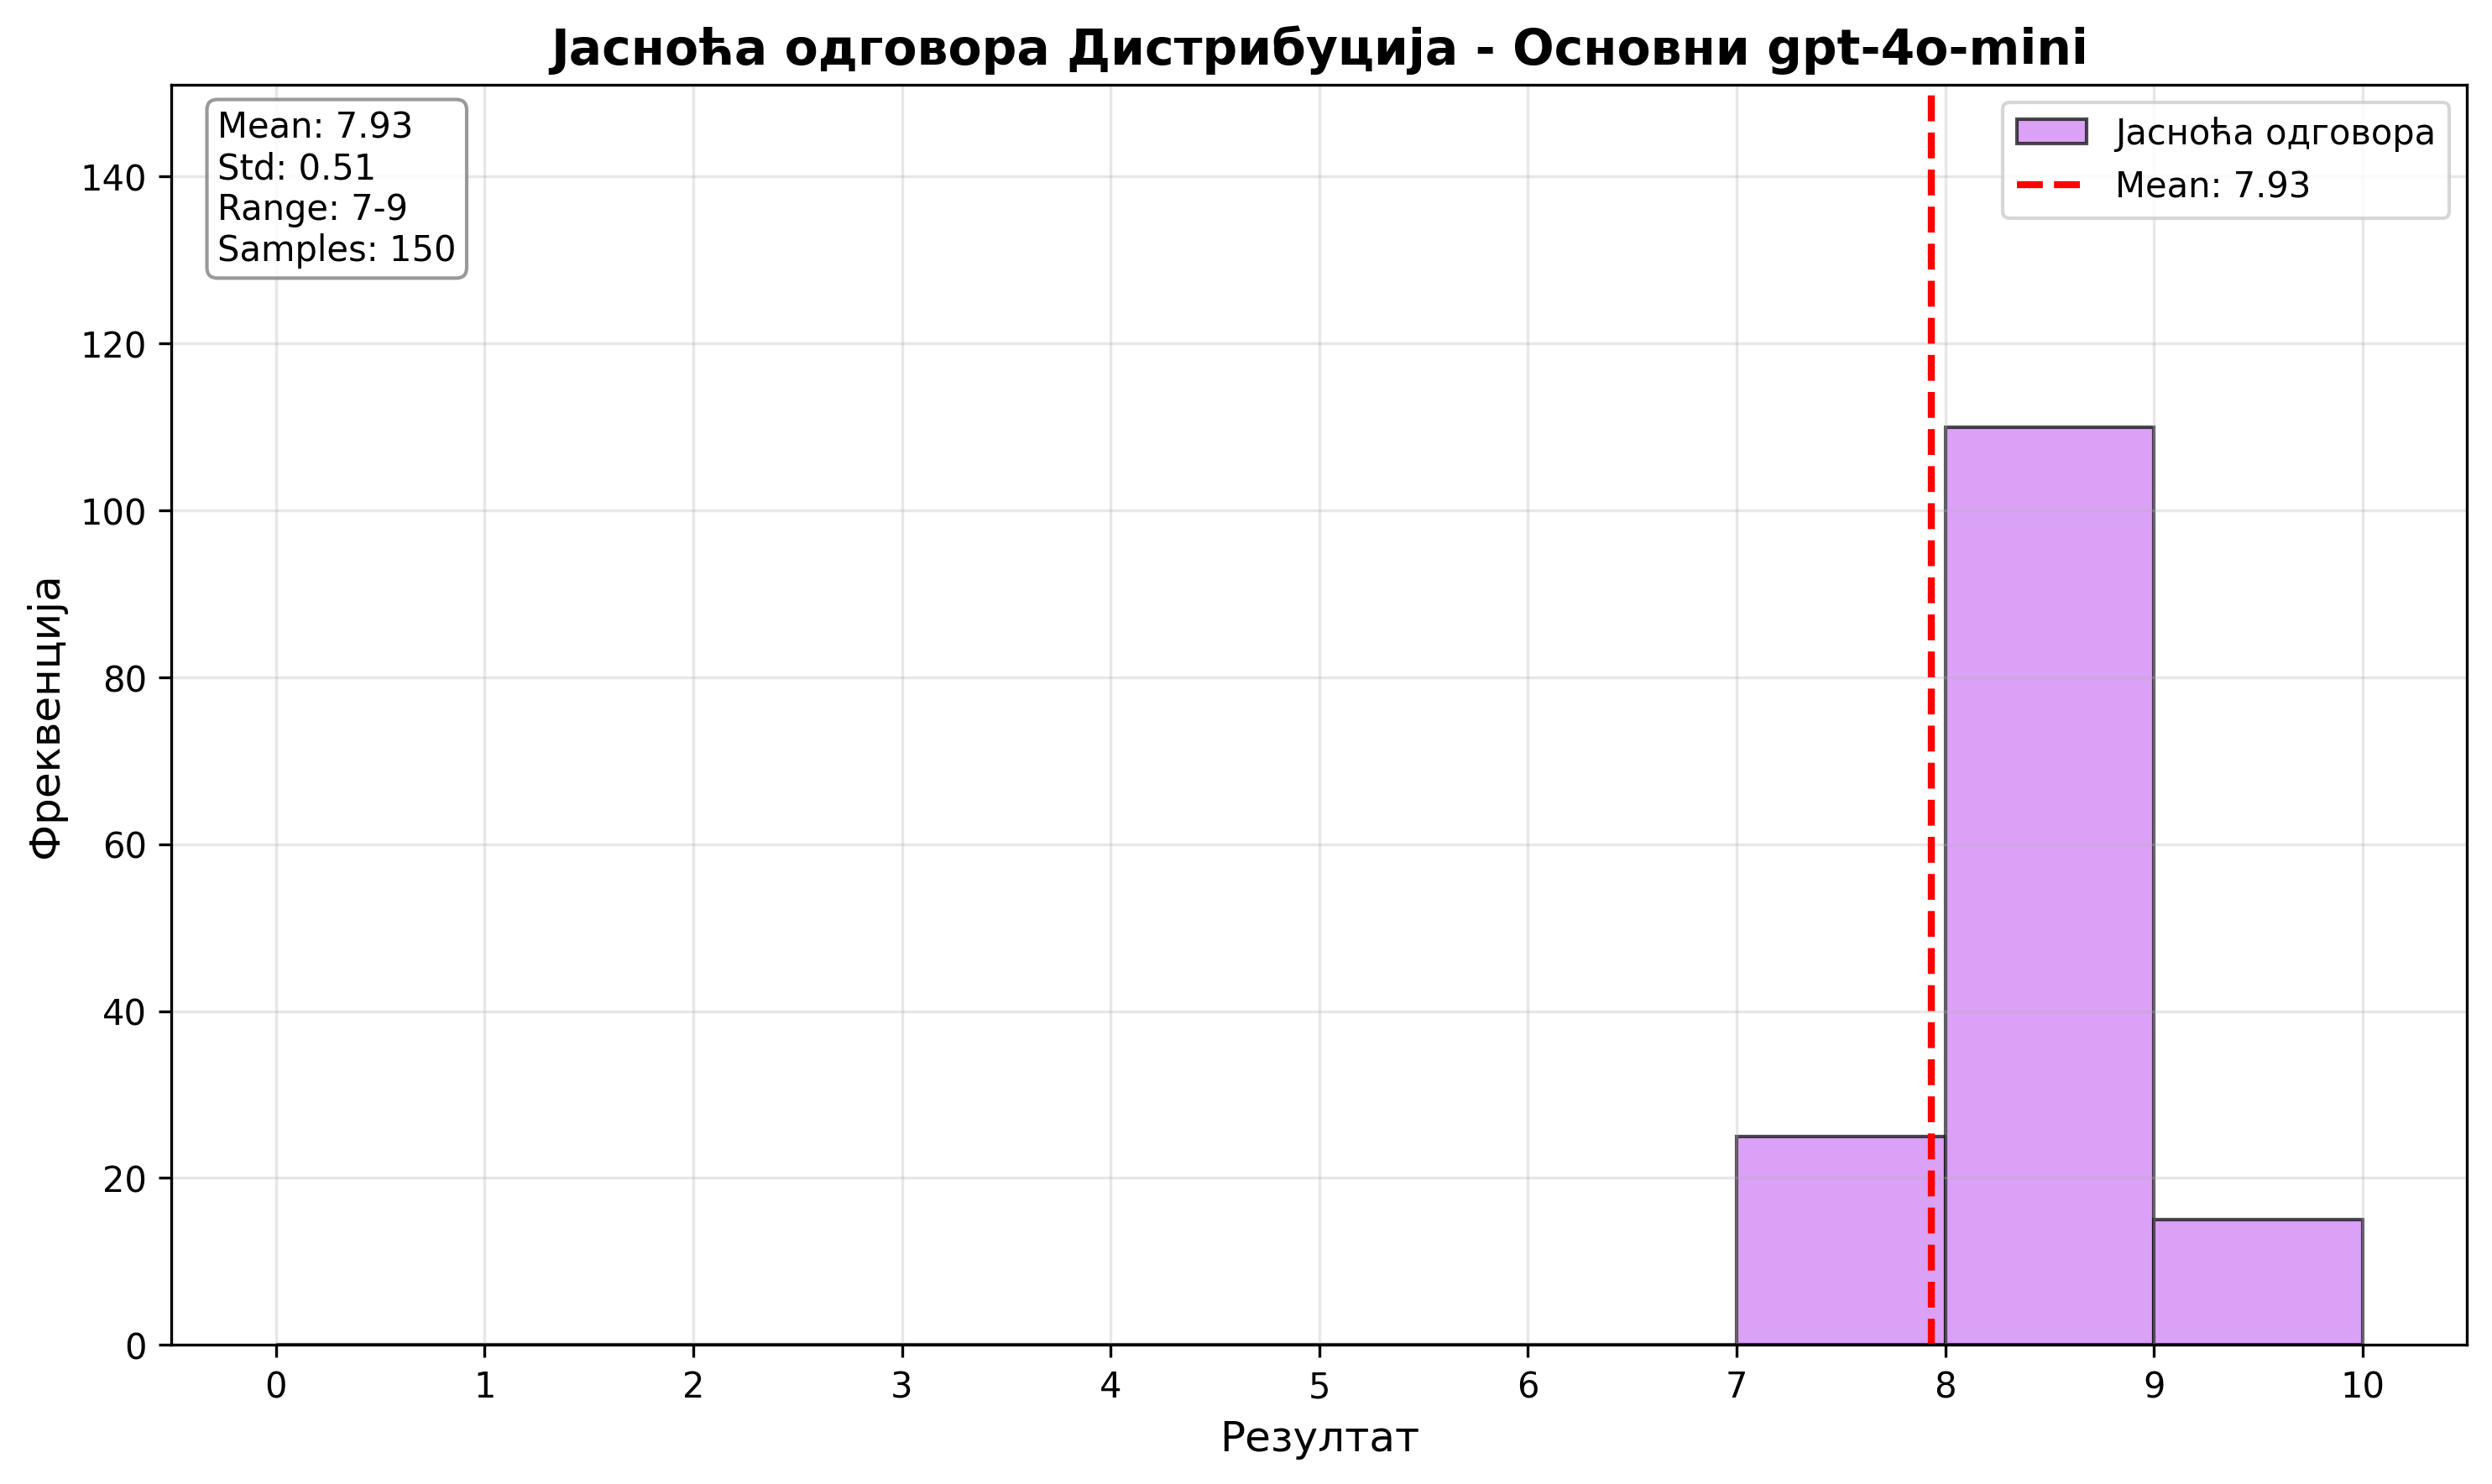
\includegraphics[width=0.8\textwidth]{images/osnovni/criteria_analysis_clarity_histogram.png}
    \caption{Хистограм анализе критеријума јасноће за основни модел}
    \label{fig:osnovni_clarity}
\end{figure}

\begin{figure}[h]
    \centering
    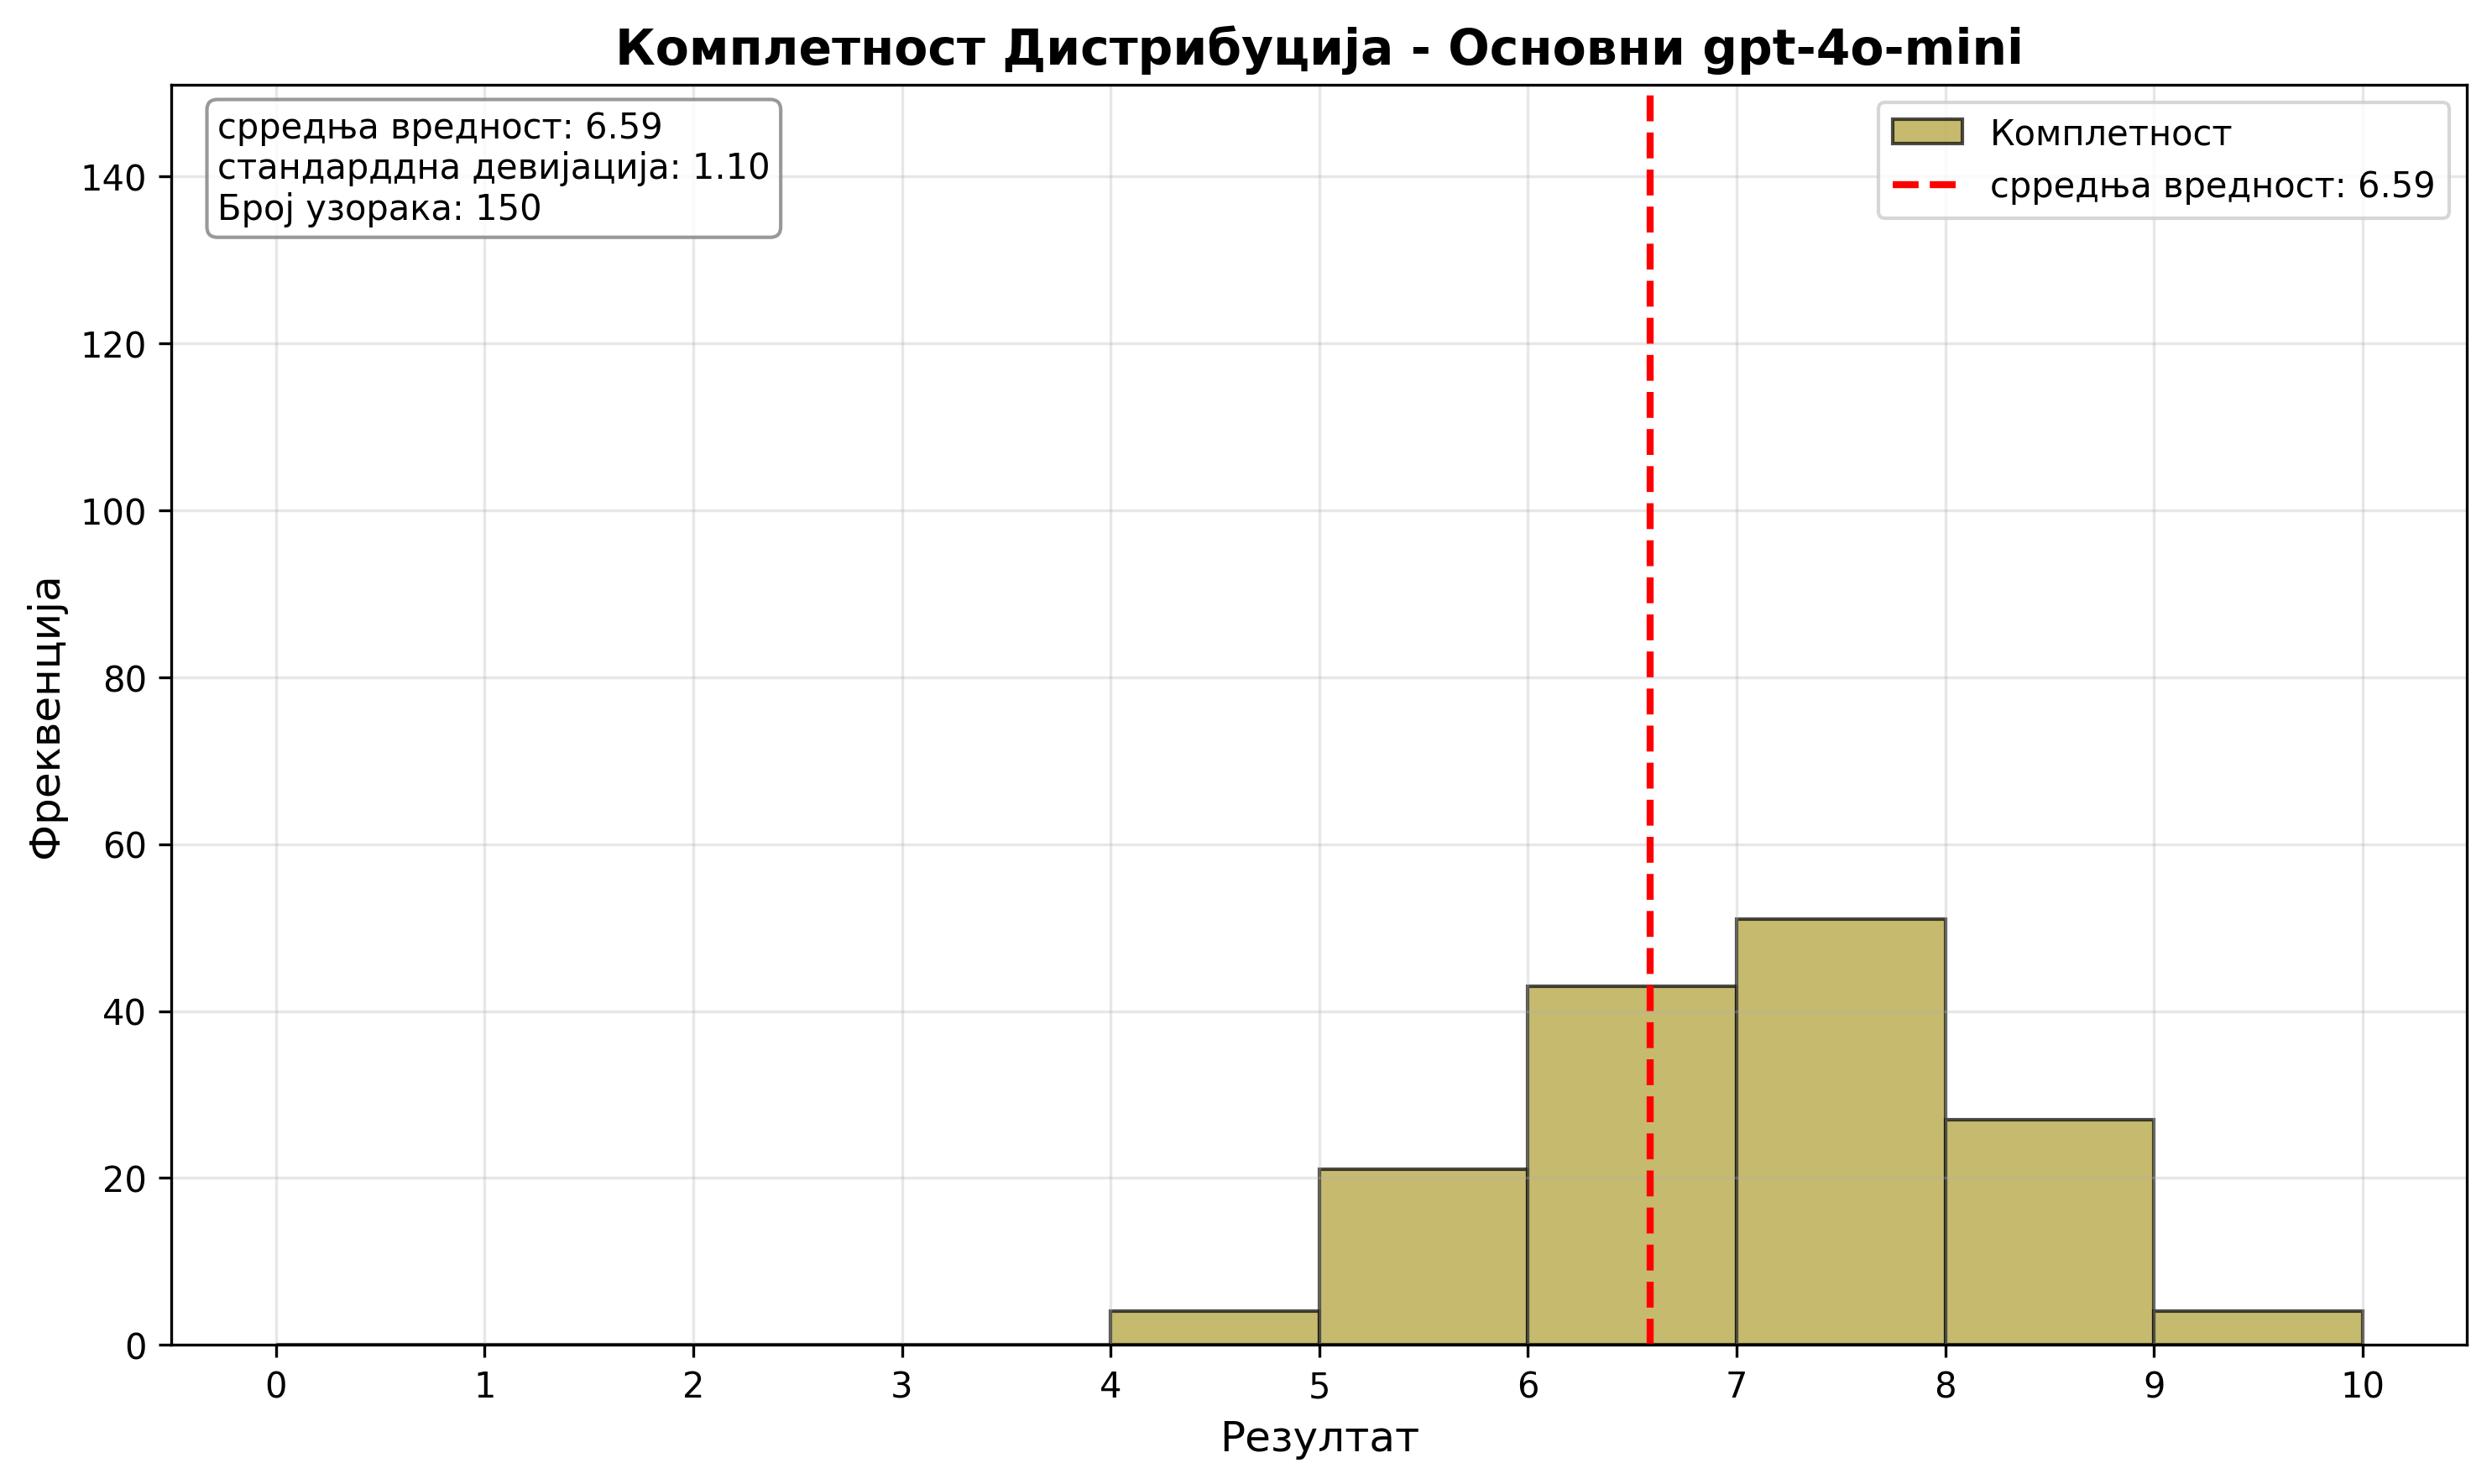
\includegraphics[width=0.8\textwidth]{images/osnovni/criteria_analysis_completeness_histogram.png}
    \caption{Хистограм анализе критеријума потпуности за основни модел}
    \label{fig:osnovni_completeness}
\end{figure}

\begin{figure}[h]
    \centering
    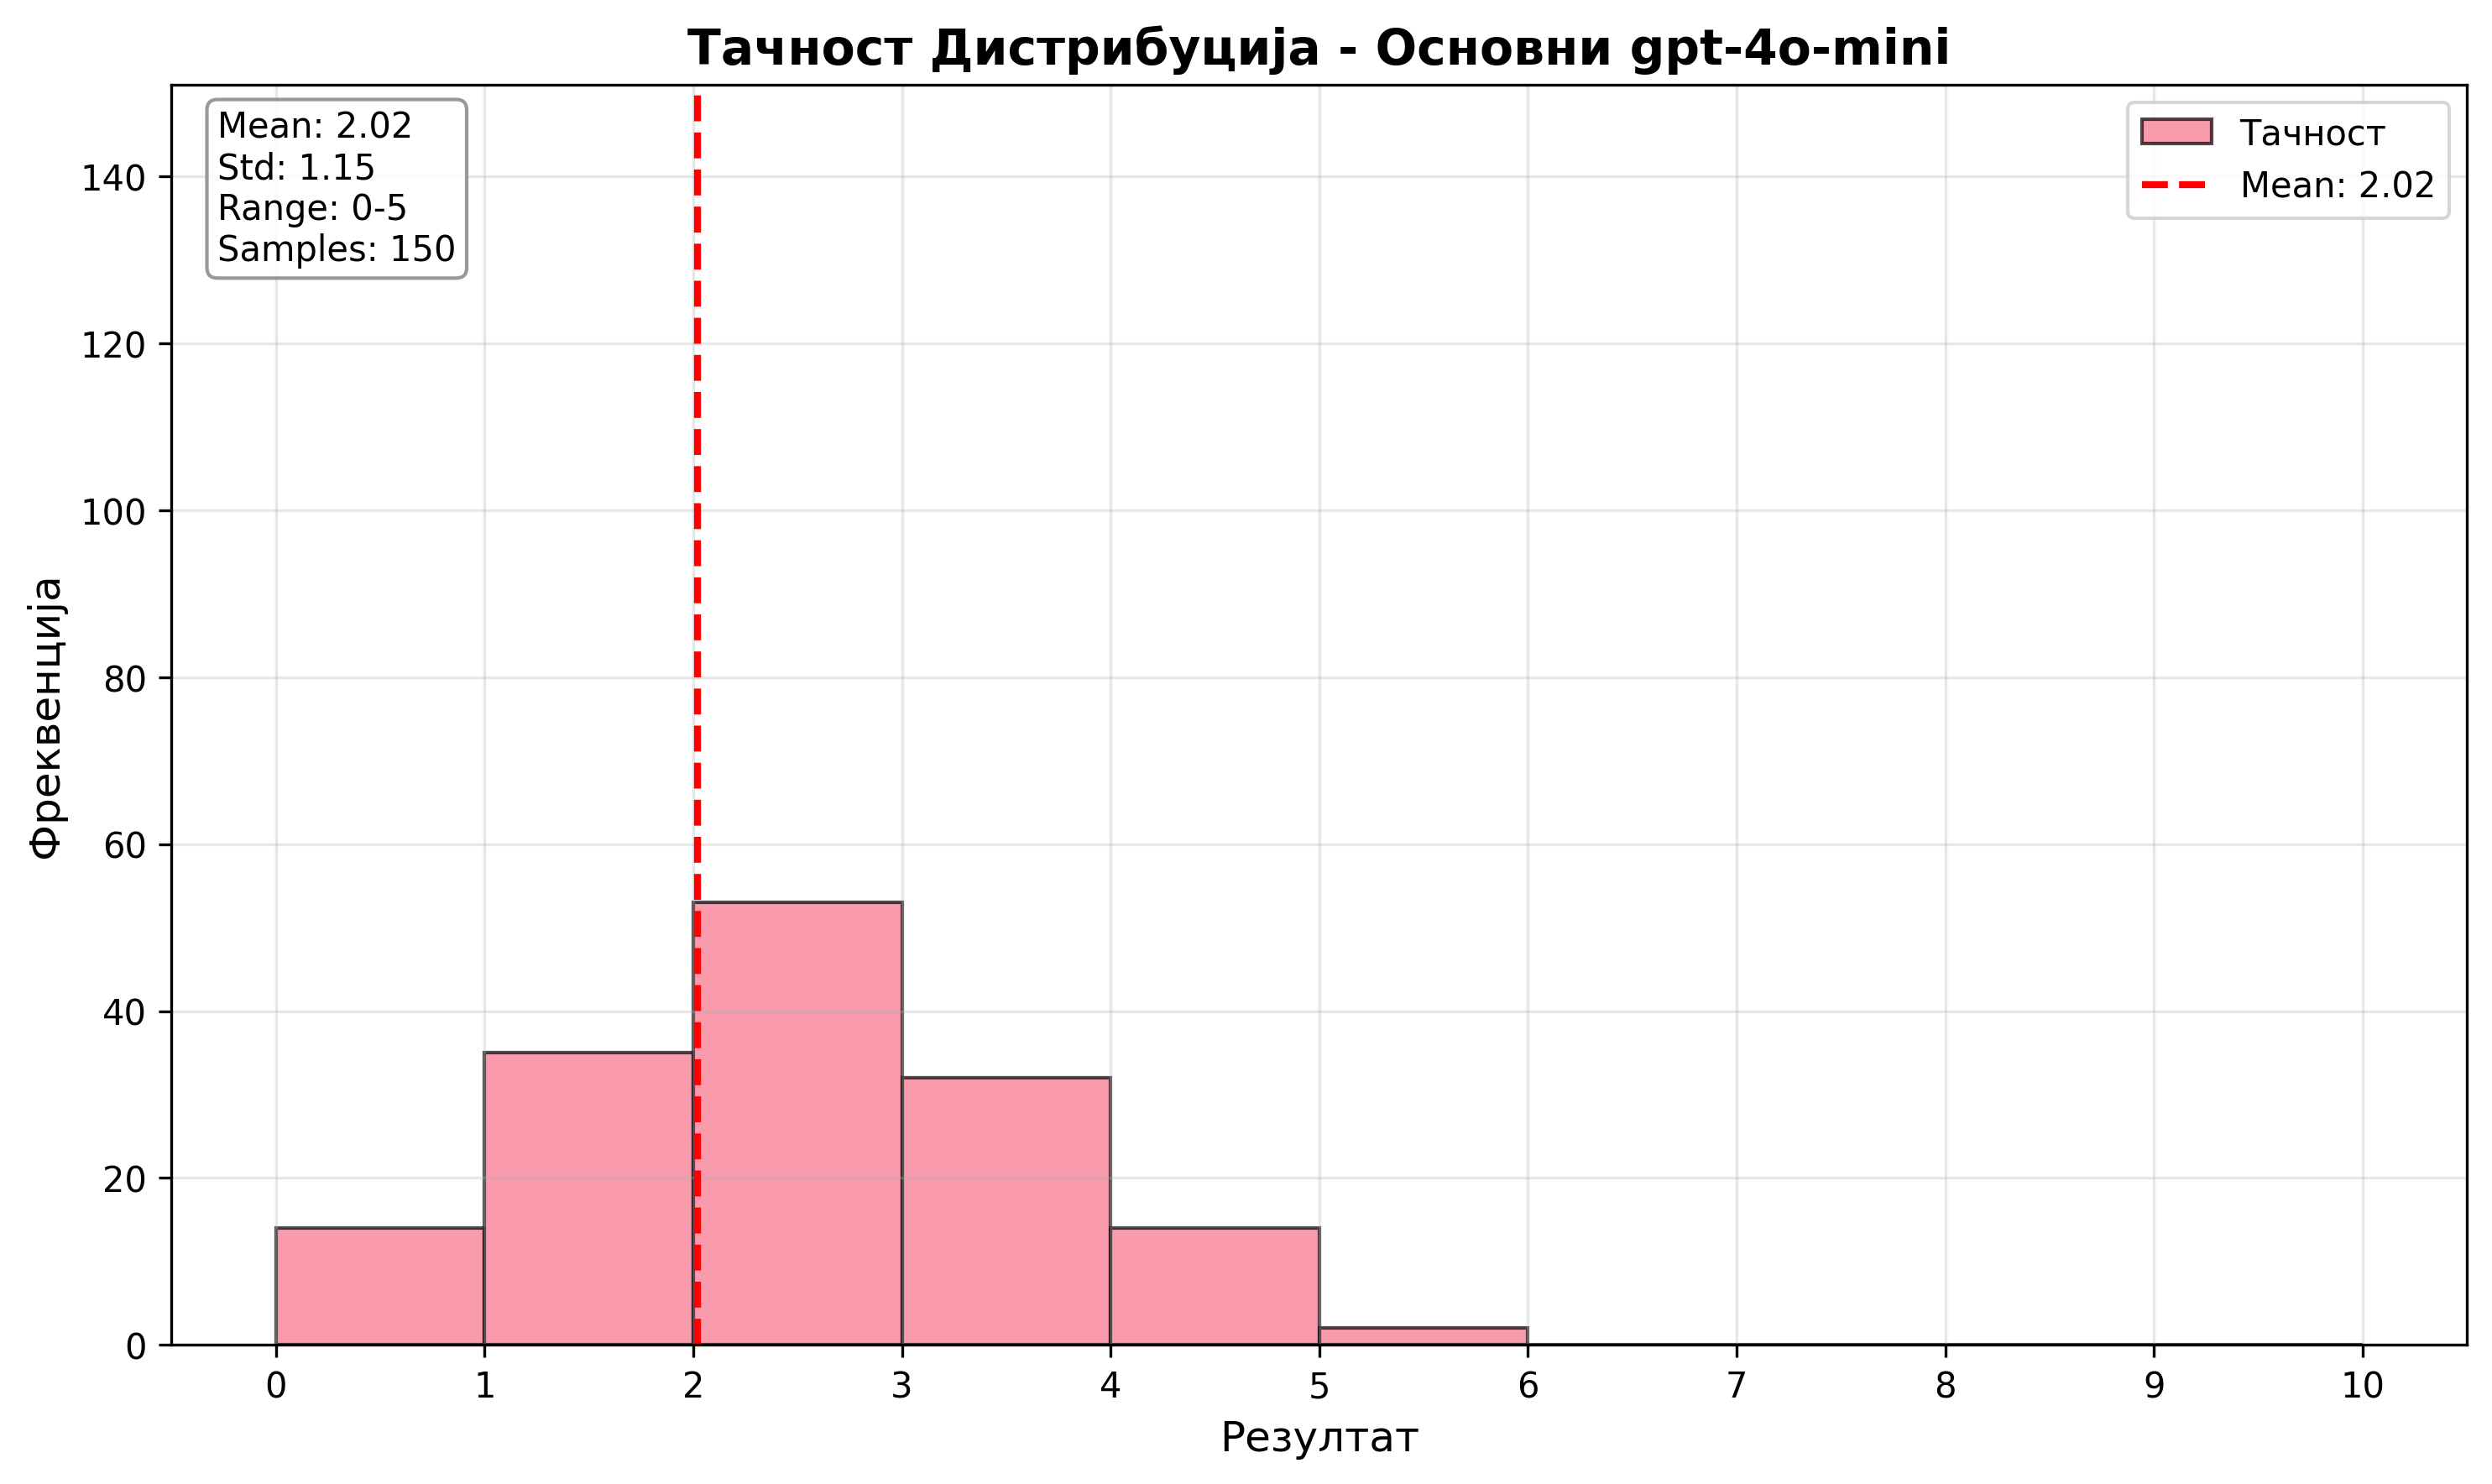
\includegraphics[width=0.8\textwidth]{images/osnovni/criteria_analysis_factual_correctness_histogram.png}
    \caption{Хистограм анализе критеријума фактичке тачности за основни модел}
    \label{fig:osnovni_factual}
\end{figure}

\begin{figure}[h]
    \centering
    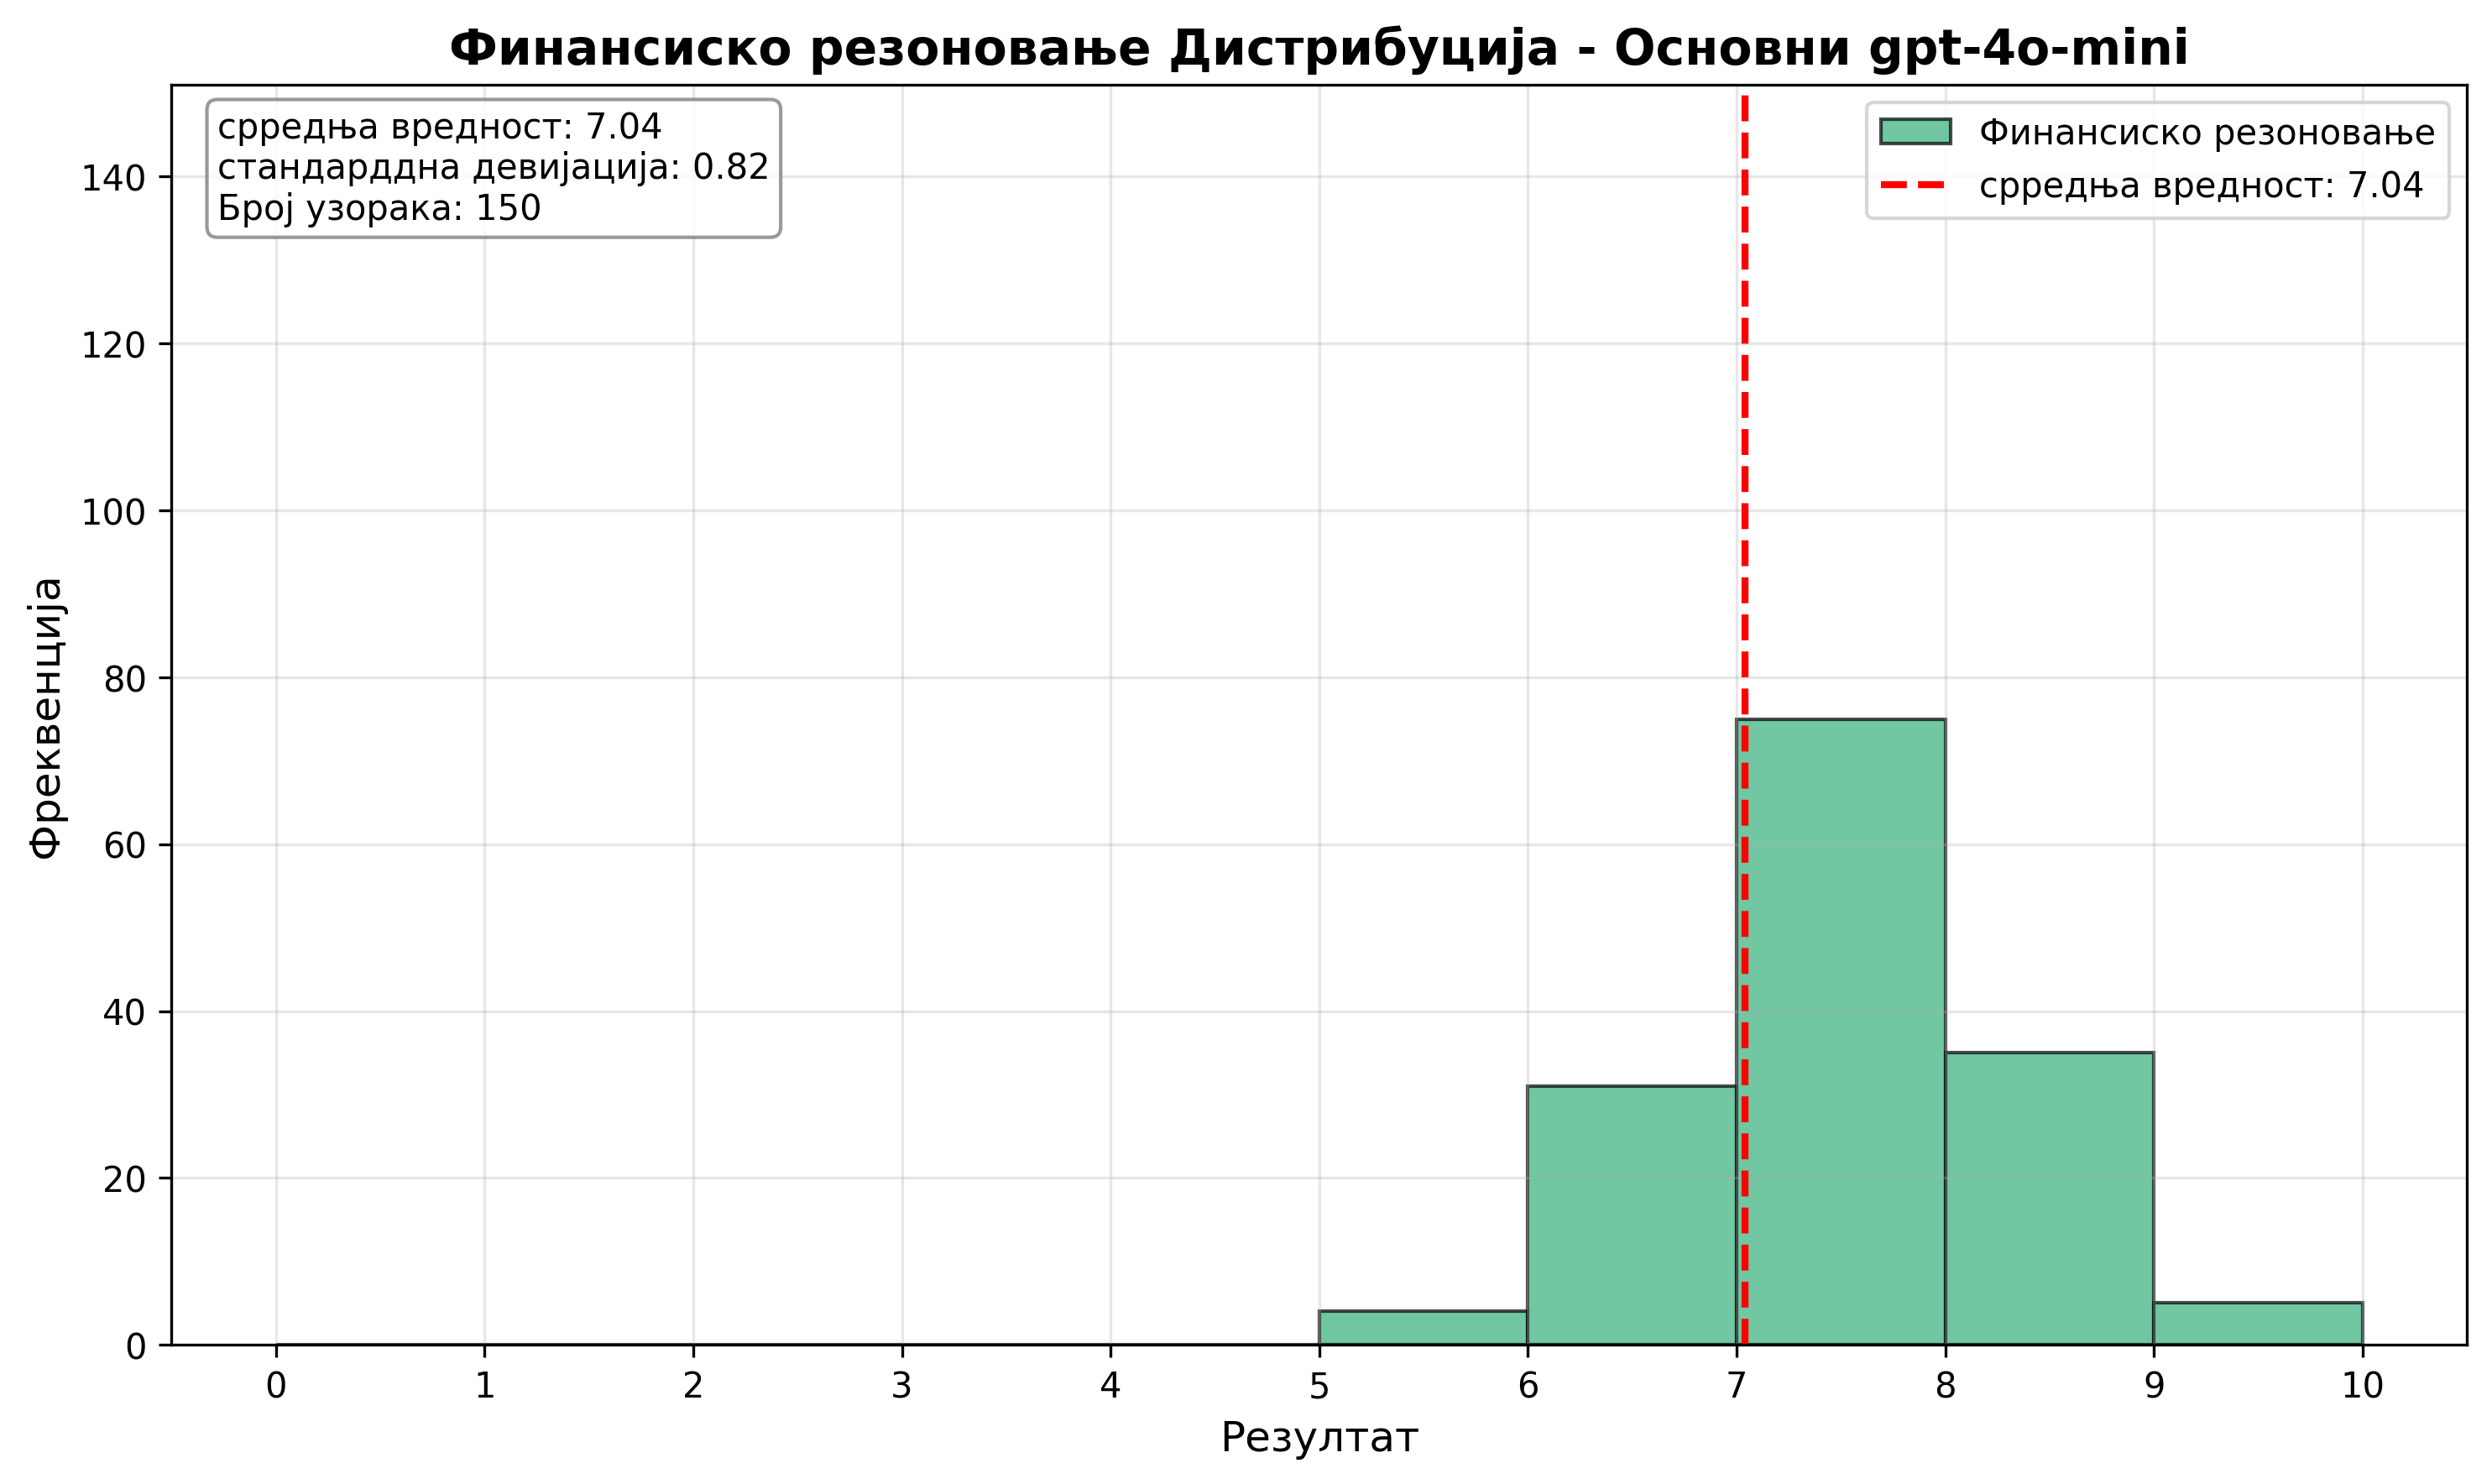
\includegraphics[width=0.8\textwidth]{images/osnovni/criteria_analysis_financial_reasoning_histogram.png}
    \caption{Хистограм анализе критеријума финансијског резоновања за основни модел}
    \label{fig:osnovni_financial}
\end{figure}

\begin{figure}[h]
    \centering
    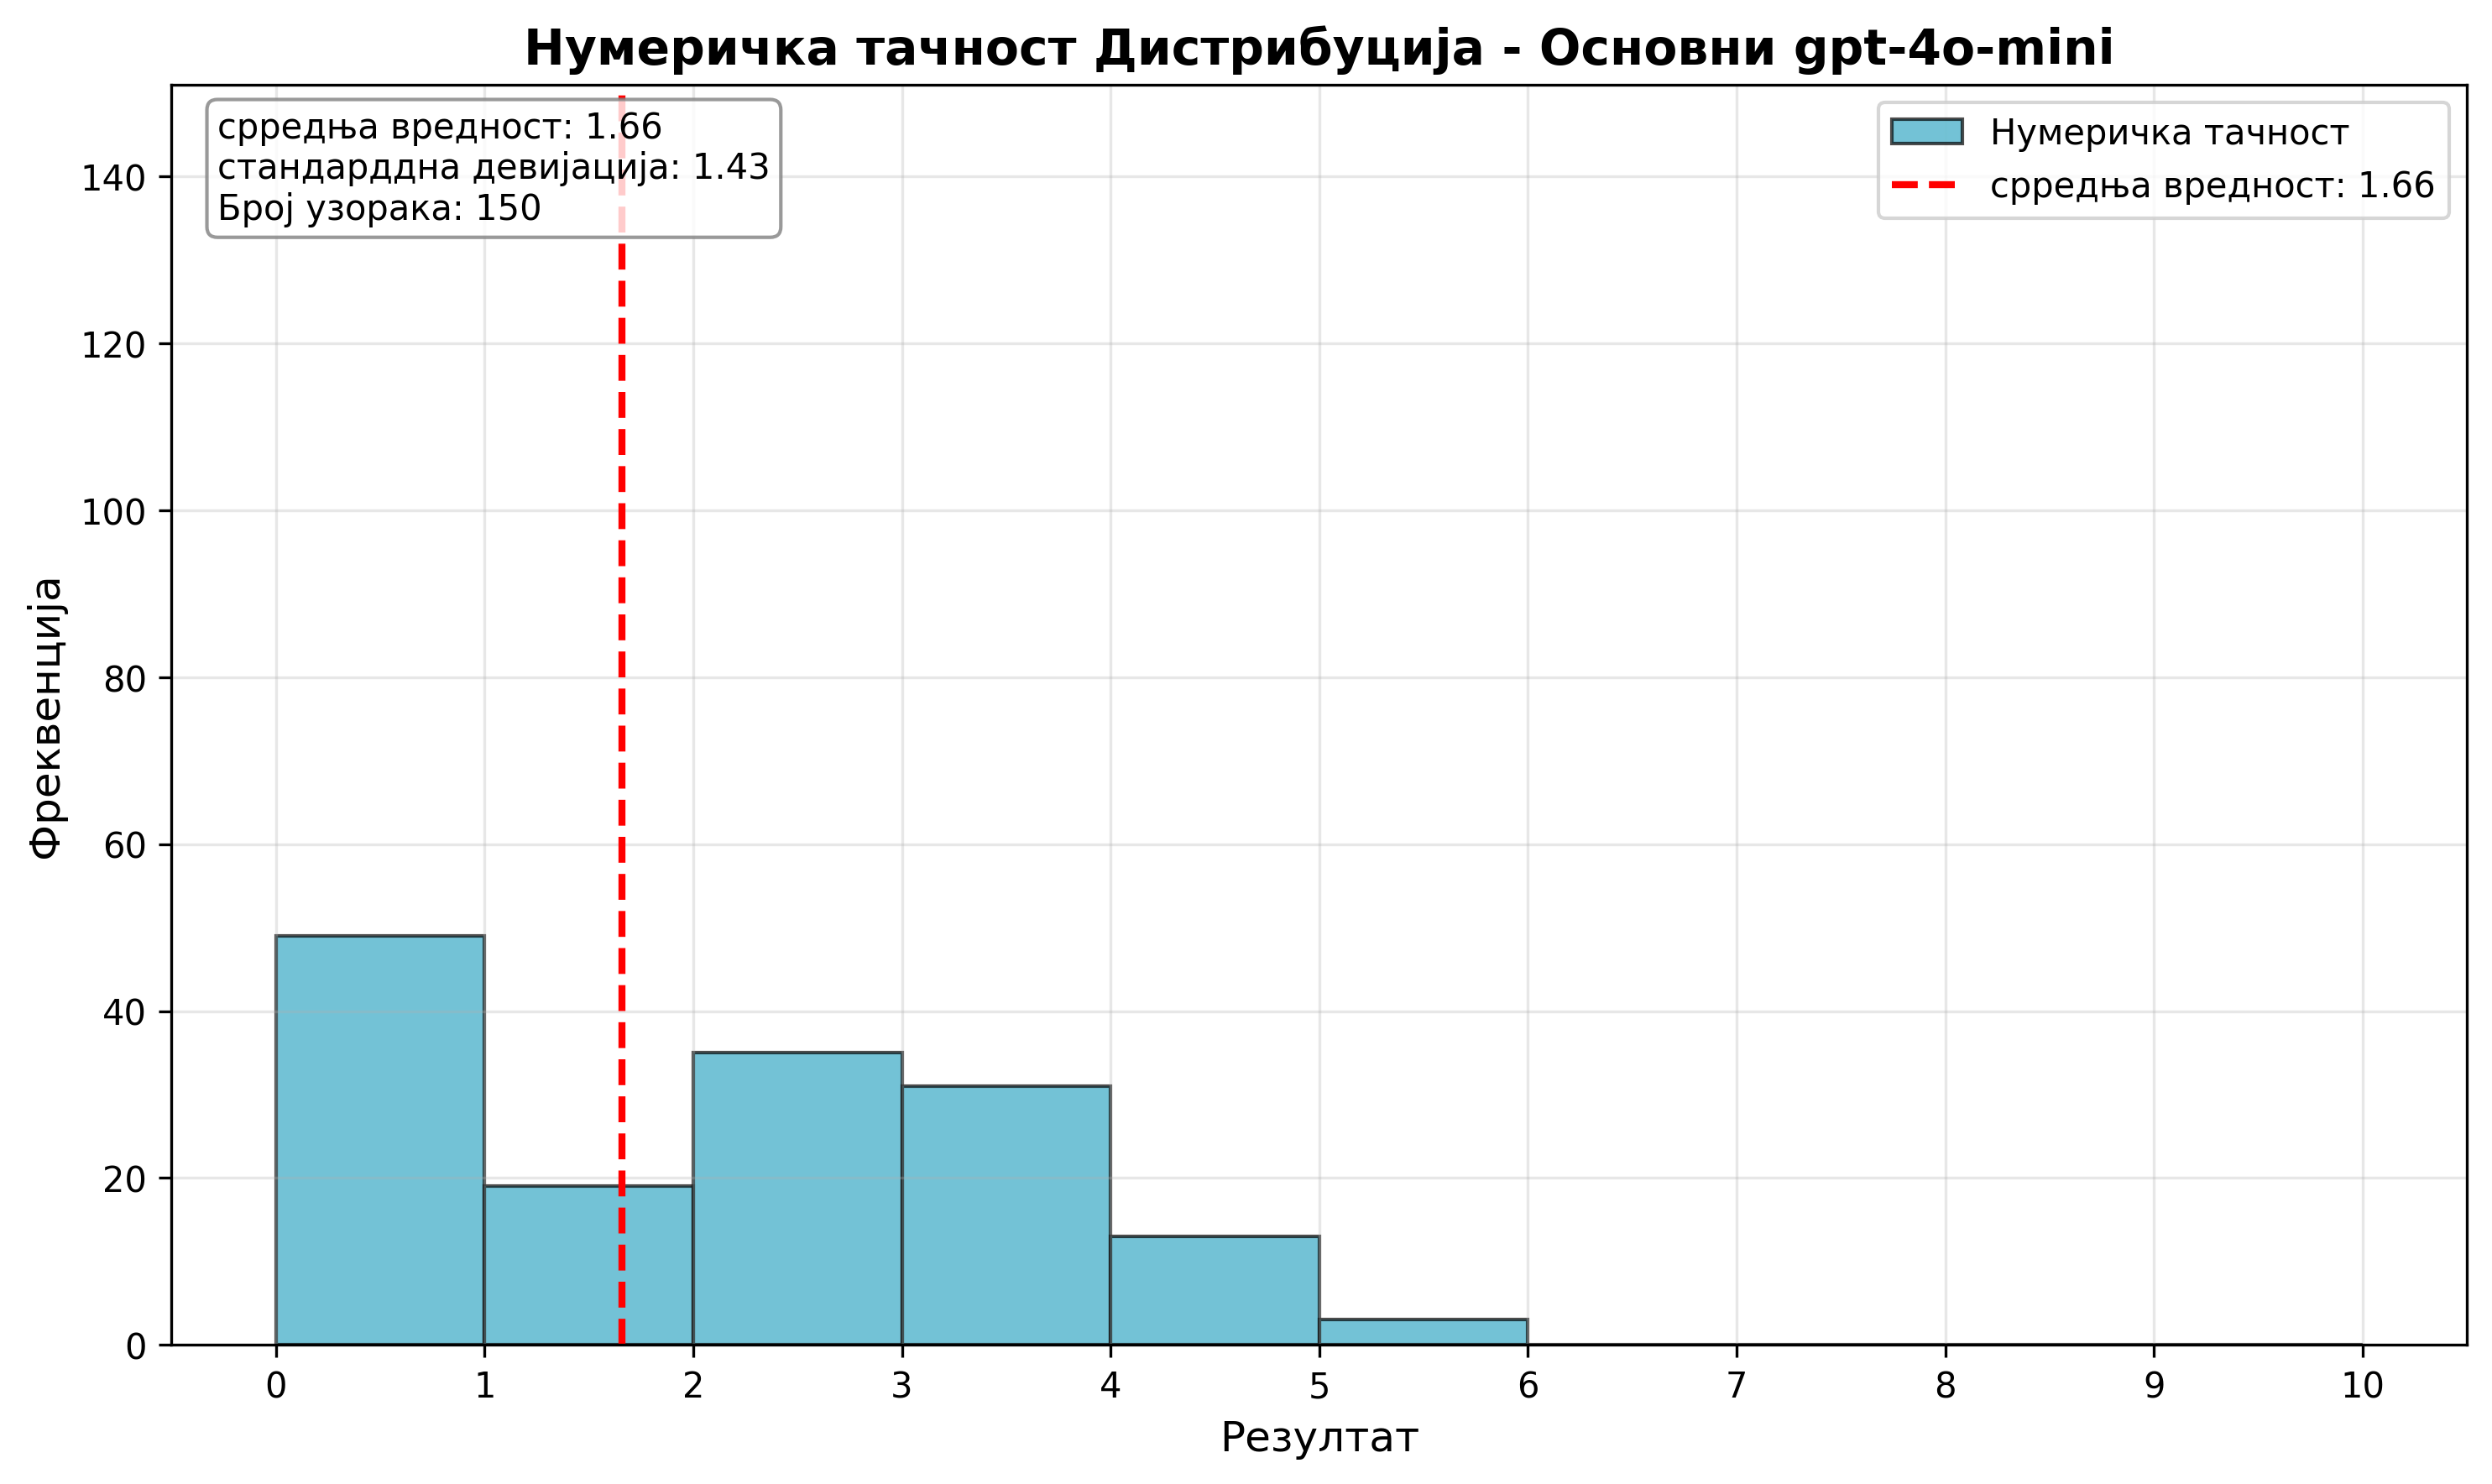
\includegraphics[width=0.8\textwidth]{images/osnovni/criteria_analysis_numerical_accuracy_histogram.png}
    \caption{Хистограм анализе критеријума нумеричке тачности за основни модел}
    \label{fig:osnovni_numerical}
\end{figure}

\section{Анализа критеријума евалуације - FinAsk модел}

Следеће фигуре приказују дистрибуцију оцена за различите критеријуме евалуације FinAsk модела:

\begin{figure}[h]
    \centering
    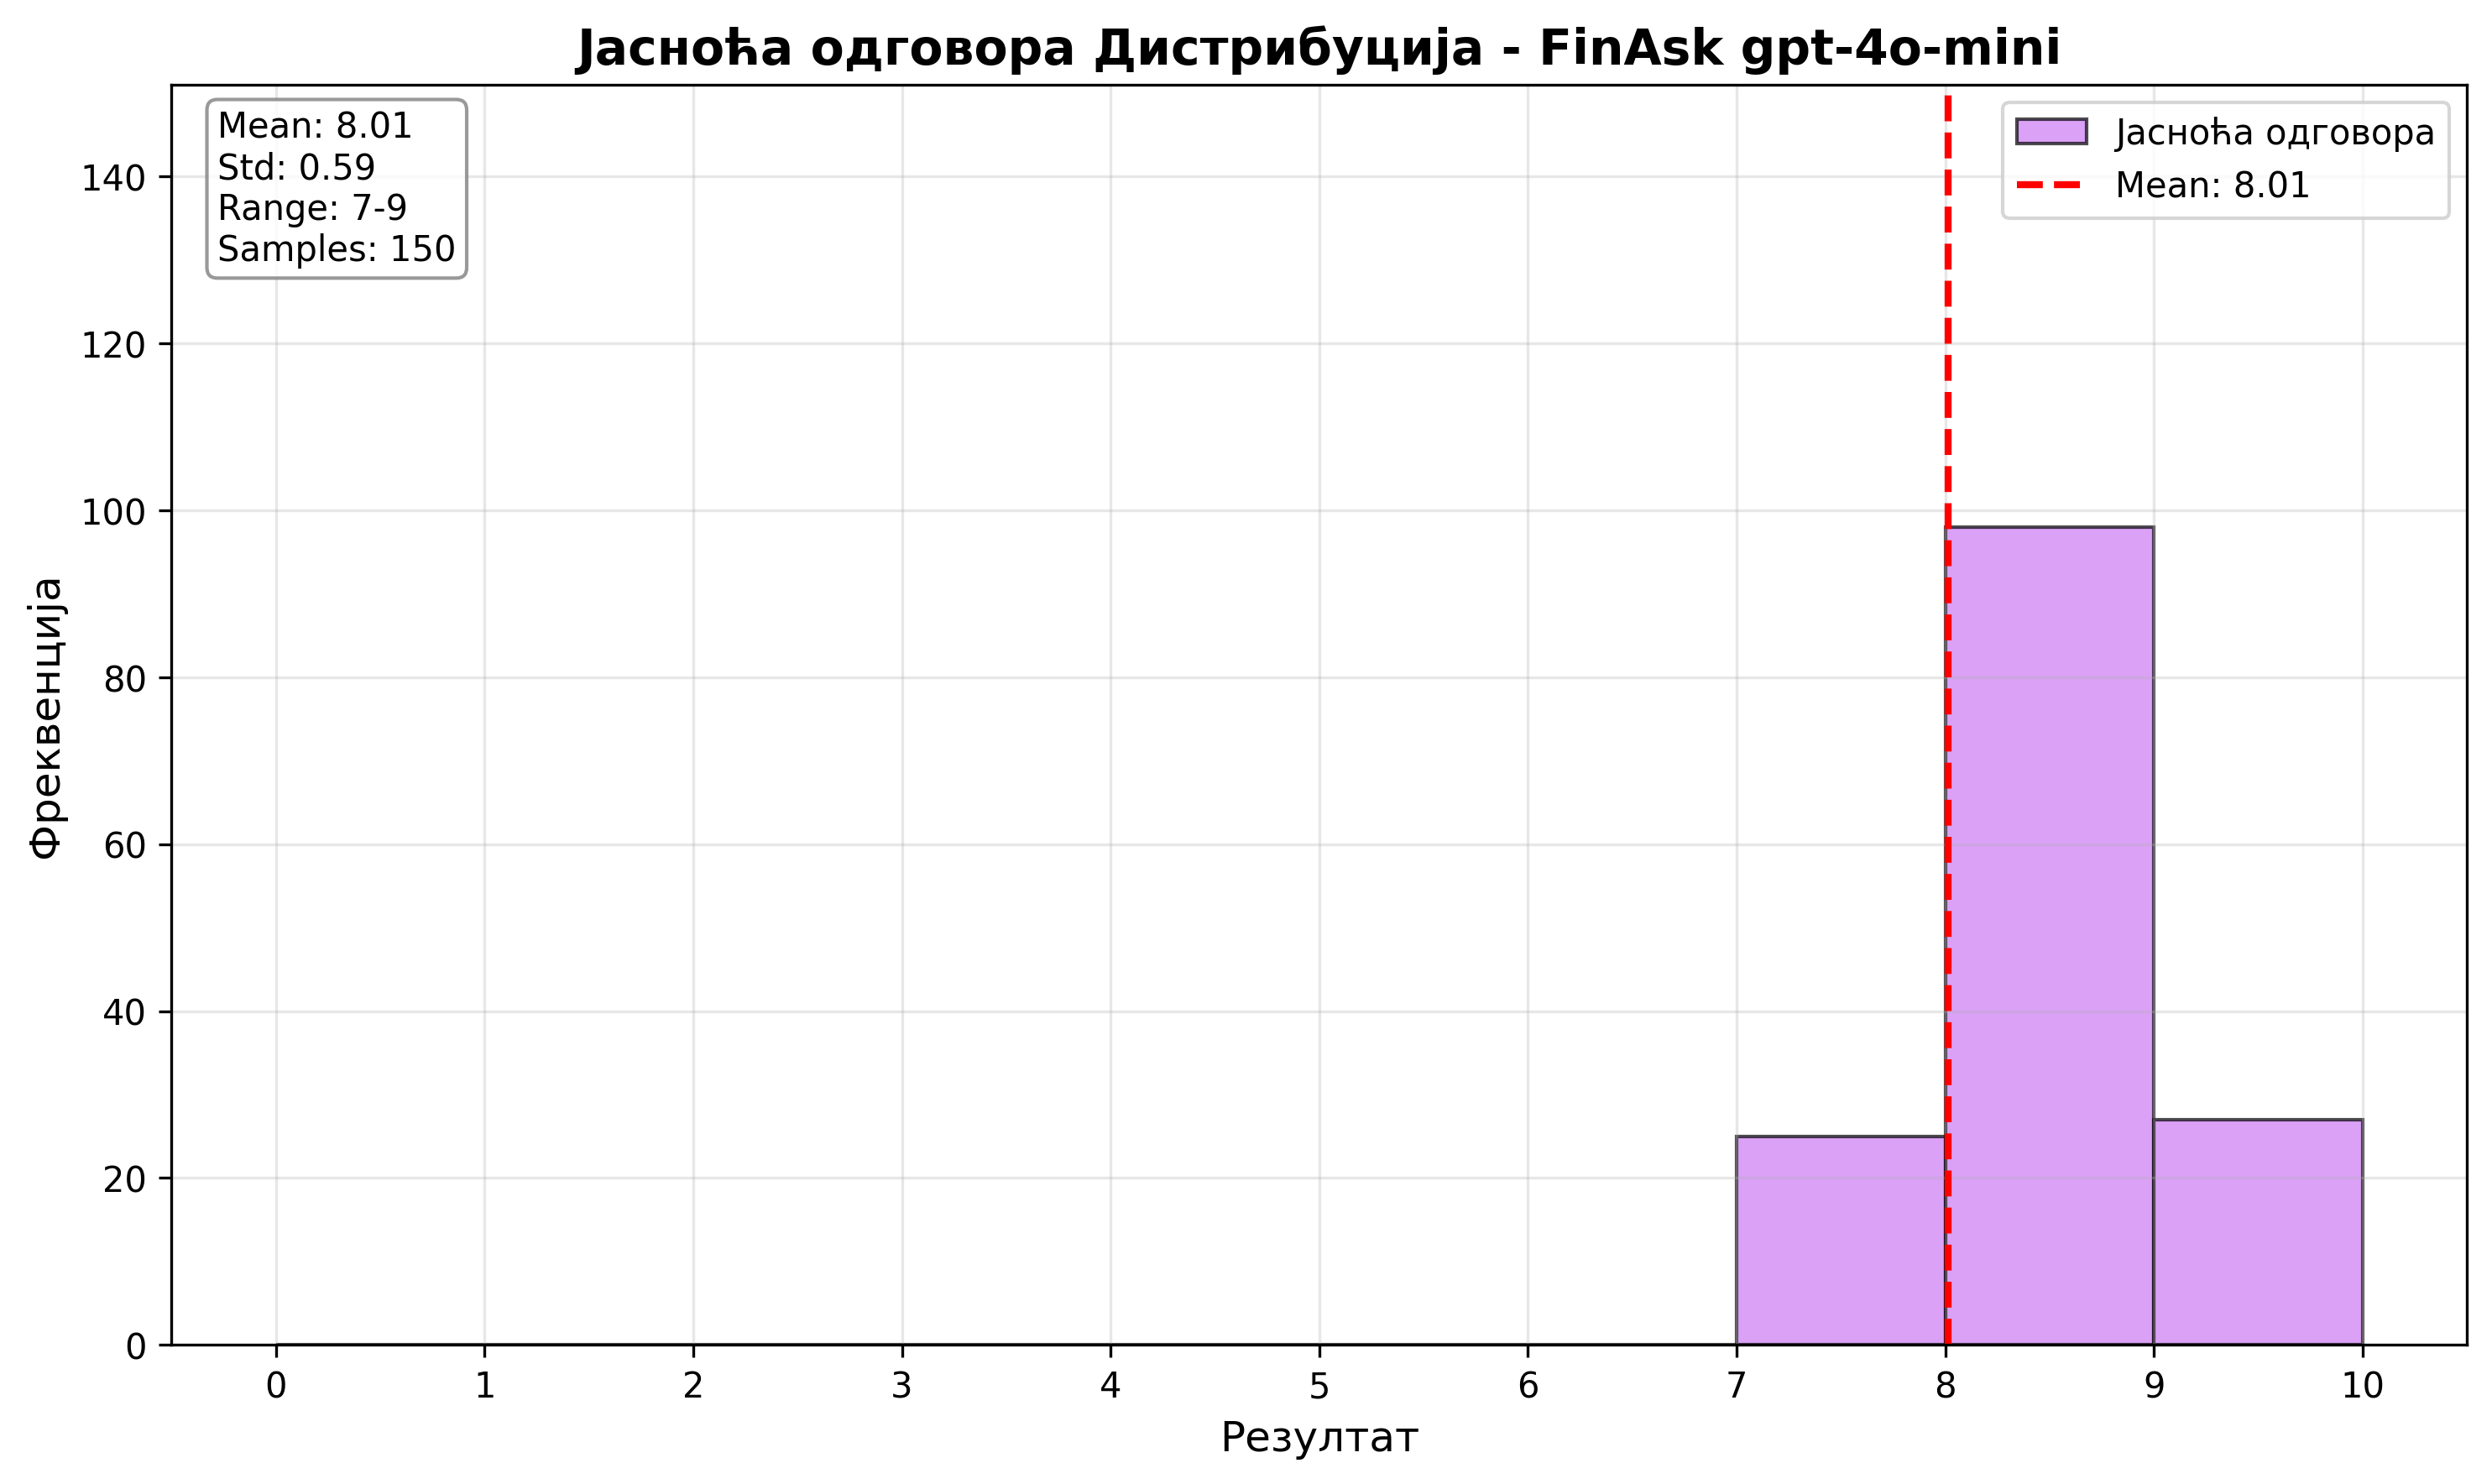
\includegraphics[width=0.8\textwidth]{images/FinAsk/criteria_analysis_clarity_histogram.png}
    \caption{Хистограм анализе критеријума јасноће за FinAsk модел}
    \label{fig:finask_clarity}
\end{figure}

\begin{figure}[h]
    \centering
    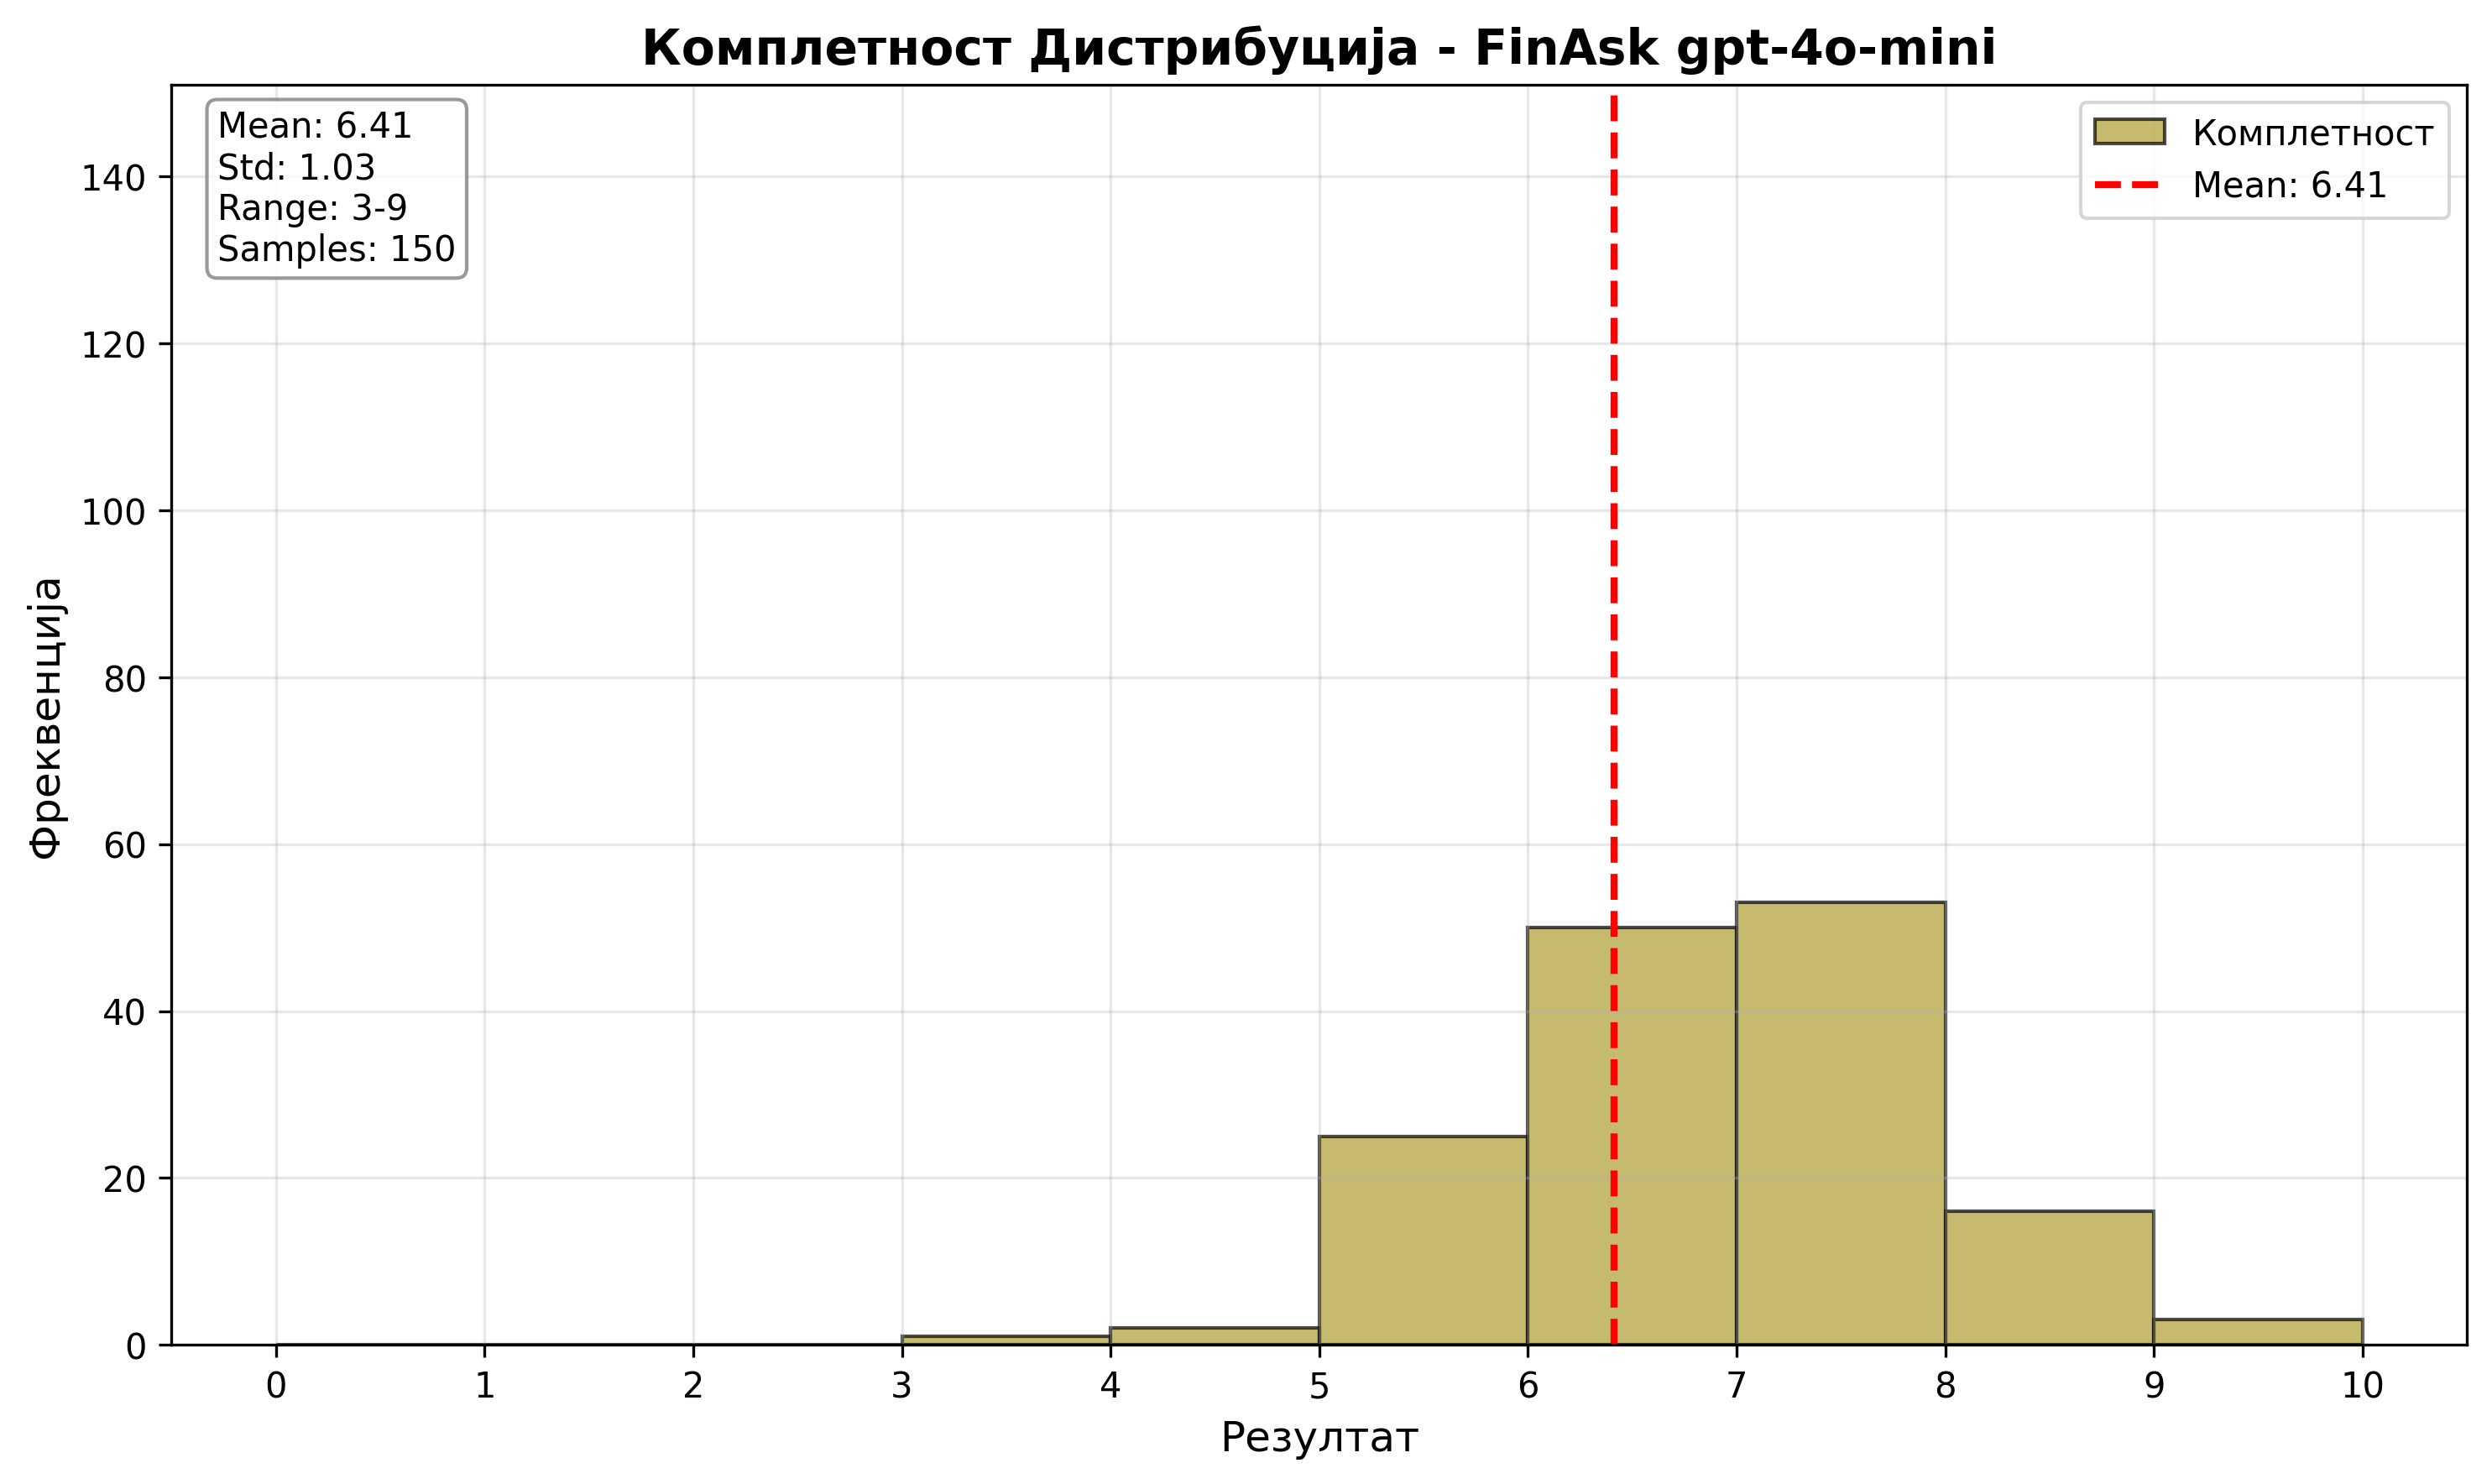
\includegraphics[width=0.8\textwidth]{images/FinAsk/criteria_analysis_completeness_histogram.png}
    \caption{Хистограм анализе критеријума потпуности за FinAsk модел}
    \label{fig:finask_completeness}
\end{figure}

\begin{figure}[h]
    \centering
    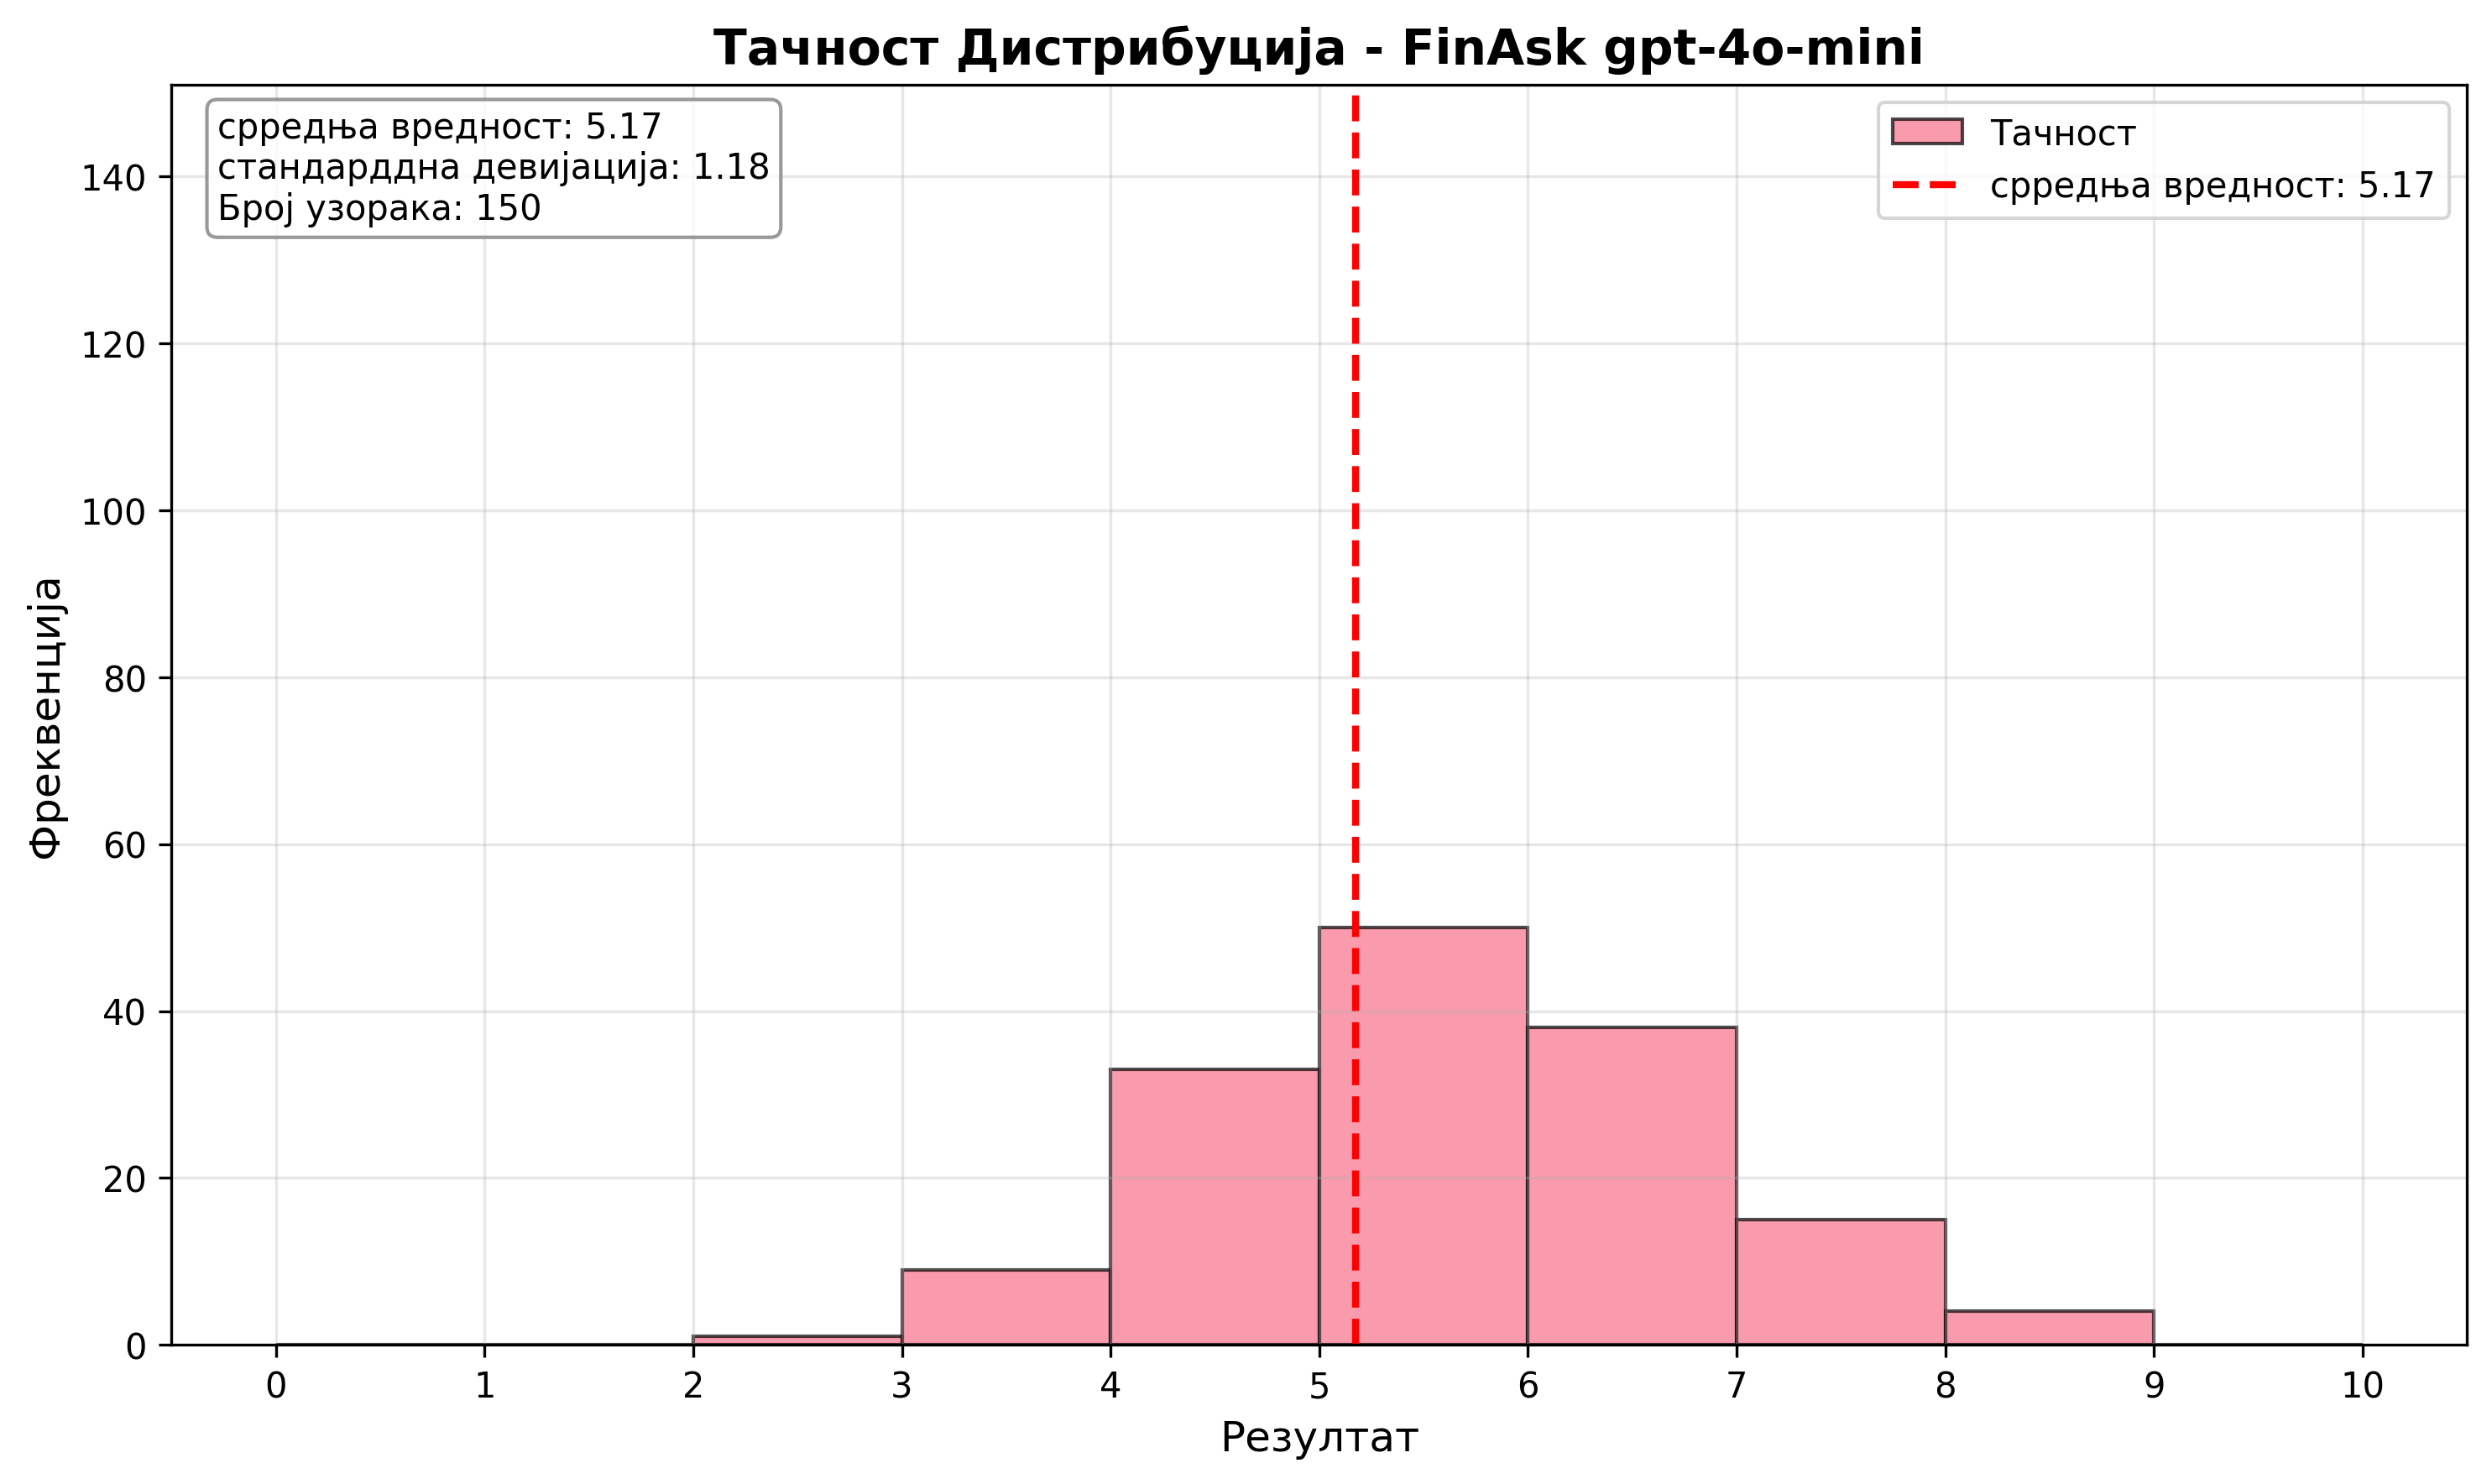
\includegraphics[width=0.8\textwidth]{images/FinAsk/criteria_analysis_factual_correctness_histogram.png}
    \caption{Хистограм анализе критеријума фактичке тачности за FinAsk модел}
    \label{fig:finask_factual}
\end{figure}

\begin{figure}[h]
    \centering
    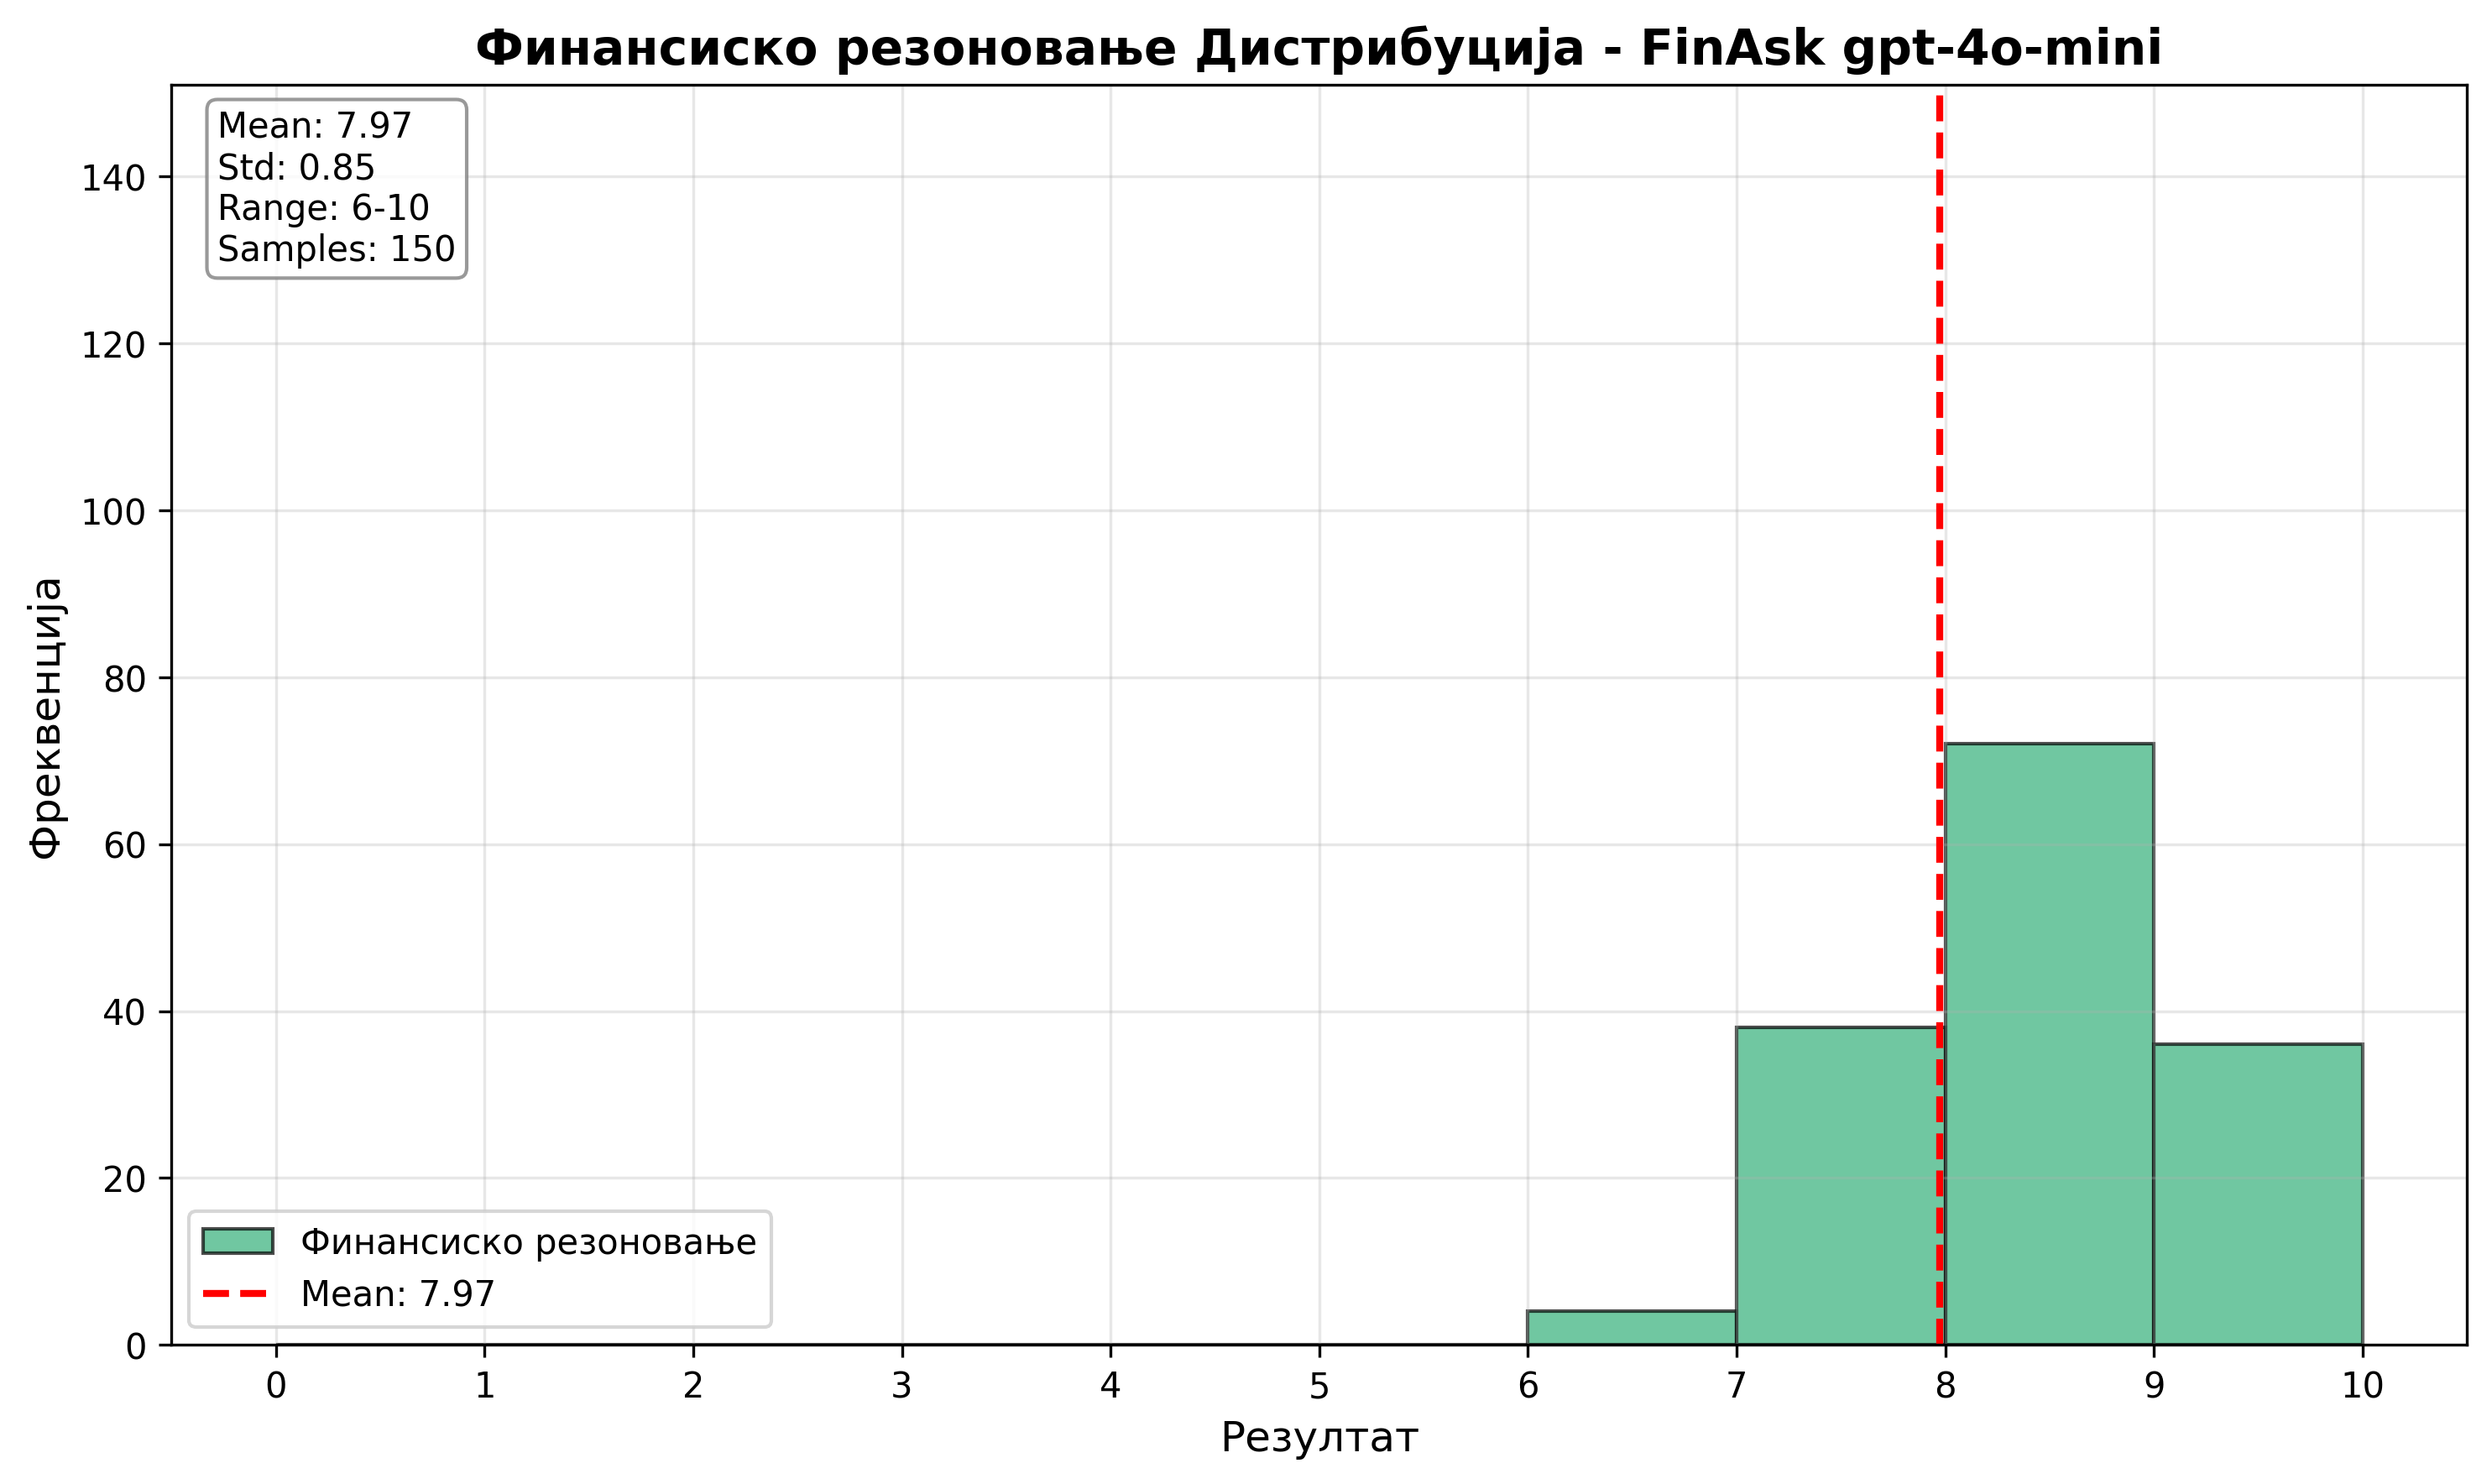
\includegraphics[width=0.8\textwidth]{images/FinAsk/criteria_analysis_financial_reasoning_histogram.png}
    \caption{Хистограм анализе критеријума финансијског резоновања за FinAsk модел}
    \label{fig:finask_financial}
\end{figure}

\begin{figure}[h]
    \centering
    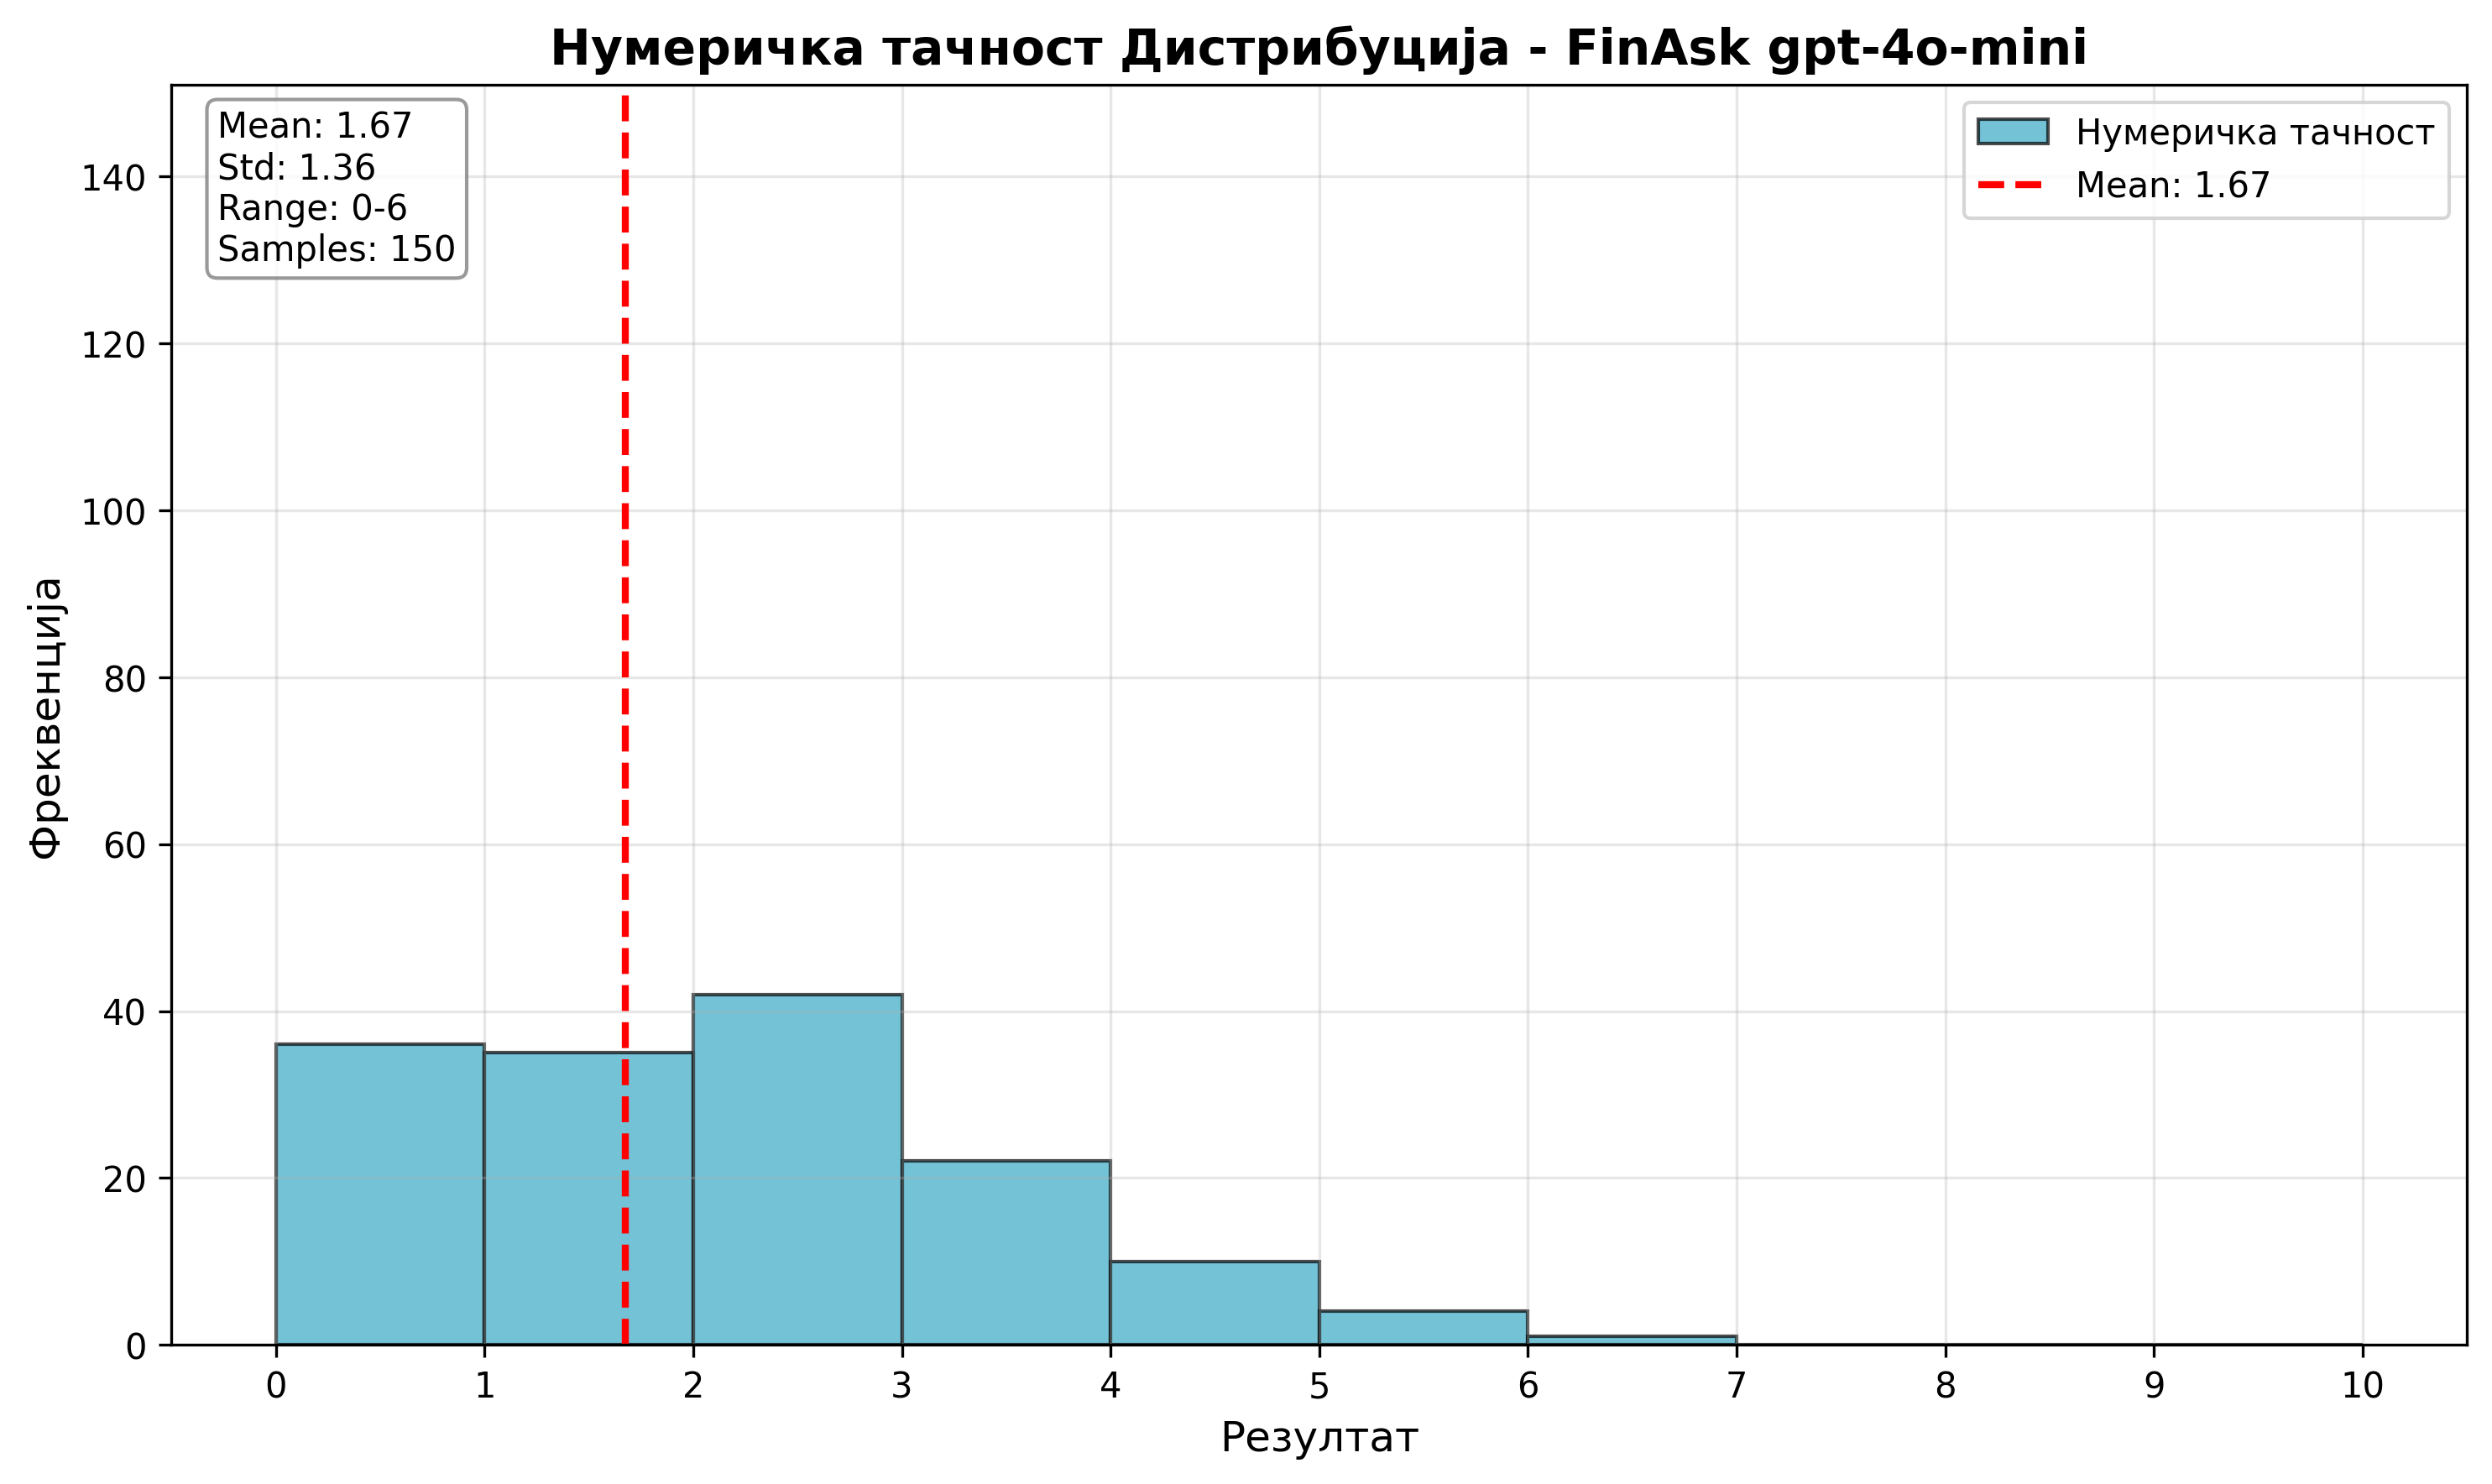
\includegraphics[width=0.8\textwidth]{images/FinAsk/criteria_analysis_numerical_accuracy_histogram.png}
    \caption{Хистограм анализе критеријума нумеричке тачности за FinAsk модел}
    \label{fig:finask_numerical}
\end{figure}

\section{Поређење резултата}

На основу приказаних хистограма, може се извршити поређење перформанси између основног модела и FinAsk модела по различитим критеријумима:

\begin{itemize}
    \item \textbf{Јасноћа (Clarity):} Поређењем фигура \ref{fig:osnovni_clarity} и \ref{fig:finask_clarity}
    \item \textbf{Потпуност (Completeness):} Поређењем фигура \ref{fig:osnovni_completeness} и \ref{fig:finask_completeness}
    \item \textbf{Фактичка тачност (Factual Correctness):} Поређењем фигура \ref{fig:osnovni_factual} и \ref{fig:finask_factual}
    \item \textbf{Финансијско резоновање (Financial Reasoning):} Поређењем фигура \ref{fig:osnovni_financial} и \ref{fig:finask_financial}
    \item \textbf{Нумеричка тачност (Numerical Accuracy):} Поређењем фигура \ref{fig:osnovni_numerical} и \ref{fig:finask_numerical}
\end{itemize}


Анализа резултата евалуације финансијског агента "Основни gpt-4o-mini" открива сложену слику перформанси система који демонстрира неуједначене способности у различитим аспектима финансијске анализе. Укупан скор од 5.80 са стандардном девијацијом од 0.54 указује на умерене перформансе са значајним варијацијама у појединачним критеријумима евалуације. Посебно је занимљива дистрибуција скорова по критеријумима, где се јасно уочава дихотомија између високих перформанси у квалитативним аспектима и изузетно слабих резултата у нумеричкој тачности.

Фактуална исправност са просечним скором од 5.09 и стандардном девијацијом од 1.26 представља умерен ниво тачности који сугерише да систем успева да идентификује и репродукује релевантне финансијске информације у приближно половини случајева. Ова метрика је кључна за практичну примену система јер директно утиче на поверење корисника и употребљивост у реалним сценаријима финансијског саветовања. Релативно висока варијабилност указује на недоследност у приступу обради различитих типова упита, што може бити последица ограничења у основном језичком моделу или недовољне оптимизације промпт инжењеринга.

Компletност одговора са скором од 6.45 демонстрира солидну способност система да пружи обухватне анализе које покривају релевантне аспекте постављених питања. Стандардна девијација од 0.97 указује на релативно конзистентну перформансу у овом домену, што сугерише да архитектура система подржава систематичан приступ структурирању одговора. Финансијско резоновање са скором од 7.96 представља један од најснажнијих аспеката система, указујући на способност извођења логичких закључака и примене финансијских принципа у анализи. Ова висока перформанса је посебно значајна јер одражава дубину разумевања финансијских концепата и способност њихове примене у различитим контекстовима.

Јасноћа комуникације са скором од 7.96 и најнижом стандардном девијацијом од 0.56 представља најконзистентнији аспект перформанси система. Ово указује на ефикасност у презентацији информација на начин који је разумљив крајњим корисницима, што је есенцијално за практичну употребљивост финансијских агената. Међутим, катастрофално слаба нумеричка тачност са скором од 1.65 и екстремно високом стандардном девијацијом од 1.47 представља критичну слабост која озбиљно компромитује употребљивост система у сценаријима који захтевају прецизне квантитативне анализе.

Ова дисхармонија између квалитативних и квантитативних способности сугерише фундаменталне ограничења у архитектури система која захтевају системске интервенције за побољшање. Висока варијабилност у нумеричкој тачности указује на непредвидивост система у хендловању математичких операција и израчуна, што представља неприхватљив ризик за финансијске апликације где је прецизност императив. Ови резултати имплицирају потребу за специјализованим модулима за нумеричку обраду и верификацију резултата пре презентације крајњим корисницима.
